% this LaTeX file was autogenerated by basicdoc.rb, do not edit
\documentclass[12pt]{book}
\usepackage[pdftex]{graphicx}
\usepackage{sidecap}
\pagestyle{myheadings}
\markboth{\hfill EasyGP version 0.1 \hfill}{\hfill EasyGP version 0.1 \hfill}
\raggedbottom
\begin{document}
\pagenumbering{roman}
\bibliographystyle{plain}
\title{EasyGP Users Manual}
\author{Dr. Richard Terry {\small MBBS FRACGP}\\
Dr. Ian Haywood {\small MBBS MPsych}}
\maketitle

\tableofcontents

\pagenumbering{arabic}
\setcounter{page}{1}

\chapter{Introduction}
\label{introduction}



\includegraphics[width=0.8\textwidth]{common/graphics/logo.png}


The purpose of this  document is to give an overview of the open source medical records project EasyGP which has been 
written initially for the Australian medical general practice environment, though it is hoped it will equally be 
applicable in other similar environments around the world. 


Written in Gambas Basic and using Postgresql as the database backend, its functionality is closely tied to 
Dr Richard Terry's original visual basic client, written way back in the dim distant past of last century in the mid 1990's. 


For several years after the year 2000,  Horst Herb (a general practitioner + IT guru),  Richard Terry  (a Newcastle GP), 
and  Ian Haywood, (a Melbourne-based psychiatry registrar) were involved with the GNUMed project, 
however it became clear after a number of years that the project was progressing in a direction that would ultimately not 
be useful to Australian general practitioners, and was relunctantly abandoned.


In 2008, Richard frustrated by the continuing poor quality of medical software in Australia stumbled upon Gambas, 
and with his background in Basic programming, deciding to take the bull by the horns, took up programming after a break of 
some years, and crafted the outline of what has become EasyGP. 


After presenting this at the nat-div 3020cc Conference in 
June 2009, a small group was formed to advance the development of the program with the ambitious goal or producing a beta 
product towards the end of 2009, or early 2010. 


\section{Hardware and OS}
\label{hardware-and-os}


Basic requirements for running EasyGP are


\begin{itemize}
\item  IBM PC compatible desktop or laptop pc.
\item  Any modern linux distribution preferably ARCH linux, Debian or Redhat
\item  Widescreen monitor preferred but not essential\end{itemize}
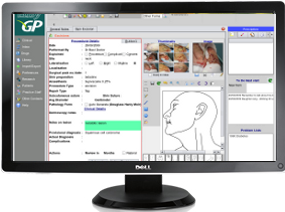
\includegraphics[width=0.8\textwidth]{gettingstarted/widescreen_lcd.png}


EasyGP has been designed to take advantage of the screen width of a modern widescreen monitor but will run quite 
happily on your laptop.

\section{Getting help}
\label{getting-help}


GPL version 3 ({\tt http://www.gnu.org/copyleft/gpl.html})

Gambas home page ({\tt http://gambas.sourceforge.net/en/main.html})

EasyGP mailing list ({\tt http://ozdocit.org/cgi-bin/mailman/admin/easygp})

PostgreSQL ({\tt http://www.postgresql.org})

Arch Linux ({\tt http:/www.archlinux.org})

ICPC2-Plus ({\tt http://www.fmrc.org.au/icpc2plus/licensing.htm})

Gambas Book - A Beginners Guide to Gambas by John Rittinghouse ({\tt http://vectorlinux.osuosl.org/Uelsk8s/gambas-beginner-guide.pdf})

Dr. Richard Terry ({\tt mailto://rterry@pacific.net.au})

Dr. Ian Haywood ({\tt mailto://ihaywood@iinet.net.au/\})

\chapter{Getting EasyGP}
\label{getting-easygp}


At the present time, you can only install a development version of EasyGP and only in a development environment of gambas 3.0 which 
may not be available as a package in your particular distribution.


Mimumum Requirements are


\begin{itemize}
\item   Linux - a distribution of your choice and a working knowledge of linux
\item   Postgresql - a working version of at least 8.3 or greater
\item   Gambas3 - development version  installed on your distribution.\end{itemize}
As there are many different ways to get this all working, if you encounter problems, please send your questions to the
 the EasyGP developers list.


see
Getting Help (see page \pageref{getting-help})











\section{Arch}
\label{arch}


No package currently exists for the development version of Gambas 3.0 in Arch so you will need to build this from the gambas3 svn. 


Either download the EasyGP source code tree by typing this at a terminal: 
svn checkout svn://ozdocit.org/easygp/trunk


or download only the necessary files described below from the source code tree at http://ozdocit.org/easygp/trunk/arch directory. 


Once these files are obtained you will need to:


\begin{itemize}
\item  Create a build directory
\item  Copy the gambas3 files into that build directory
\item  Change the name of PKGBUILD.gambas3 to PKGBUILD
\item  Build the package by typing makepkg (or makepkg --asroot)
\item  Install the package the usual way using pacman e.g pacman -U gambas3-svn-pkgnumber.tar.gz\end{itemize}


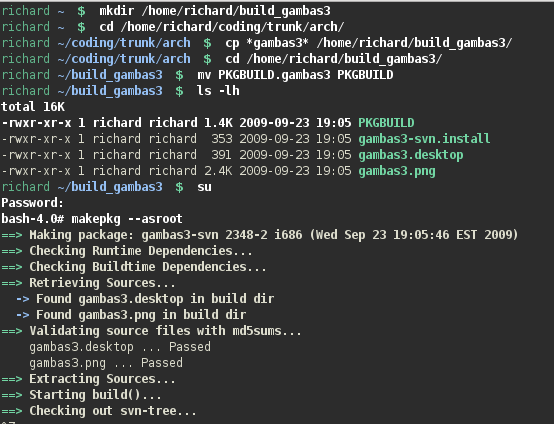
\includegraphics[width=0.8\textwidth]{gettingstarted/archlinux-build-gambas.png}




Once gambas3 has been built, you may run this, locate your downloaded EasyGP svn and run this as a project, or if you've not yet downloaded 
the easygp svn, you can create an svn project from within gambas itself.


see 
Downloading EasyGP (see page \pageref{downloading-easygp})

\section{Debian}
\label{debian}
\section{Redhat}
\label{redhat}


\section{Downloading EasyGP}
\label{downloading-easygp}


Currently EasyGP is only available via SVN. The repository is at 
\begin{verbatim}
svn://ozdocit.org/easygp/trunk
\end{verbatim}






\begin{figure}[ht] 
\begin{minipage}[b]{0.3\linewidth} 
\centering 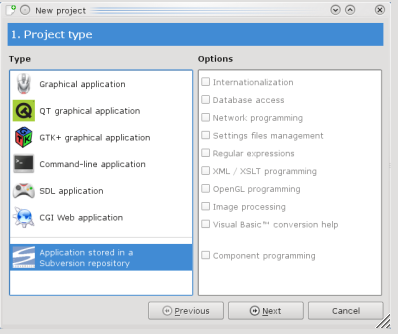
\includegraphics[width=\linewidth]{gettingstarted/createprojectsvn.png}
\end{minipage}
\hspace{0.5cm}
\begin{minipage}[b]{0.65\linewidth}


\begin{itemize}
\item  Fire up gambas3
\item  Select new project
\item  Select the option of downloading from an svn repository
\item  Click the Next button\end{itemize}

\end{minipage}
\end{figure}




\begin{figure}[ht] 
\begin{minipage}[b]{0.3\linewidth} 
\centering 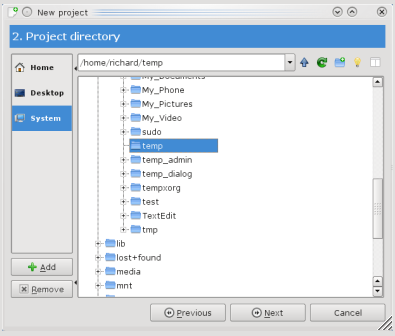
\includegraphics[width=\linewidth]{gettingstarted/createprojectdir.png}
\end{minipage}
\hspace{0.5cm}
\begin{minipage}[b]{0.65\linewidth}


\begin{itemize}
\item  Select the directory you wish to store the code in
\item  Click the Next button on the project creation wizard to continue.
\end{itemize}

\end{minipage}
\end{figure}


\begin{figure}[ht] 
\begin{minipage}[b]{0.3\linewidth} 
\centering 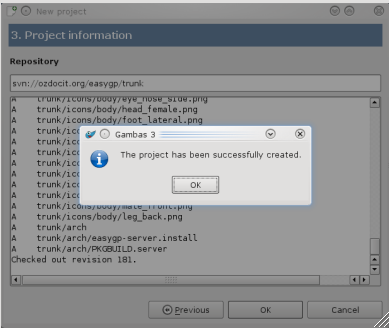
\includegraphics[width=\linewidth]{gettingstarted/createprojectdownload.png}
\end{minipage}
\hspace{0.5cm}
\begin{minipage}[b]{0.65\linewidth}
\begin{itemize}
\item  Copy and paste or type in the svn address and hit return 
\item  Watch gambas create the project
\item  Be patient as download from the internet can take some time.
\end{itemize}

\end{minipage}
\end{figure}




\section{Building your database}
\label{building-your-database}






Eventually database packages will be available for the common distros.


\subsection{Manual build of database}
\label{manual-build-of-database}


If there isn't a database package for your distro (currently, that's everyone)
you can build a database directly from SQL sources in the SVN repository.
First you need to install 
PostgreSQL ({\tt http://postgresql.org/}) for your system. Please see your distros documentation for this and ensure that the postmaster
is running and test that you can create and view databases using 
pgAdmin ({\tt http://www.pgadmin.org/})  before proceeding. All distros will have packages for pgAdmin3.


Next, download the SVN (as above), and fire up a shell. Go to the `trunk' directory
downloaded by SVN and then the `db' subdirectory. There run the install script:


\begin{verbatim}
./install-easygp.sh
\end{verbatim}


This should install a working database for most sensible setups of PostgreSQL. The
script will ask you to enter your root password (for Ubuntu that's your user password)
and then an administrator's password for the EasyGP database. (ideally this should
be different to the root password). The administrator user is always called `easygp'.
The console output should be similar to the one shown below.




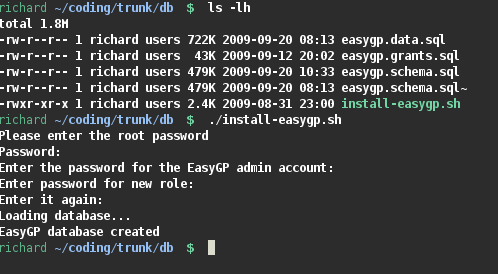
\includegraphics[width=0.8\textwidth]{gettingstarted/console.png}


Note it is impossible to cover every possible Postgres setup and somebody is bound to
have this script fail on them. If that happens please send a bug report with the 
contents of the file `/tmp/easygp-errors'. You may encounter non-critical errors for example if 
you have manually used the dropdb command in a terminal but not removed the easygp or staff role.


Once you've built the database, you can check it if you like using pgAdmin.


To run easygp you have two options
\begin{itemize}
\item  If using the SVN go to the startup folder and set modStartup as the startup form
\item  If running an executable simply execute easygp.gambas.\end{itemize}
As this will be the first time the program has run, as setup wizard will appear.


\section{Setup Wizard}
\label{setup-wizard}


If the database has been successfully built, a default user called 'easygp' will have been created. 
If you inspect the database using pgAdmin, it should look something similar to this:


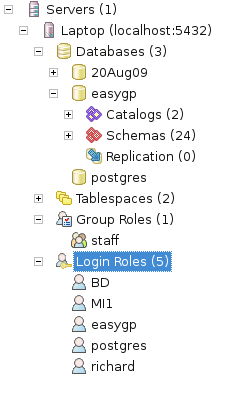
\includegraphics[width=0.8\textwidth]{gettingstarted/pgadmin-users.png}




The user 'easygp' has the permissions necessary to allow you to access the EasyGP database, to add your general practice 
as a new organisation and to create a system administrator.


Note the user 'easygp' is not and will never be a  'staff member' and as such cannot run the clinical sections of the program. 


After the database wizard has been run, you should logon as 'easygp' or the sysadmin you created, and enter any further 
staff members (see page \pageref{staff-members}) or 
organisations (see page \pageref{organisations}) that you wish.


\subsection{ Using the Wizard}
\label{using-the-wizard}
Our setup wizard will hopefully make it easy for you to create your general practice organisation 
and add your initial system admin  user. If not, please let us know how to improve it!


\begin{figure}[ht] 
\begin{minipage}[b]{0.3\linewidth} 
\centering 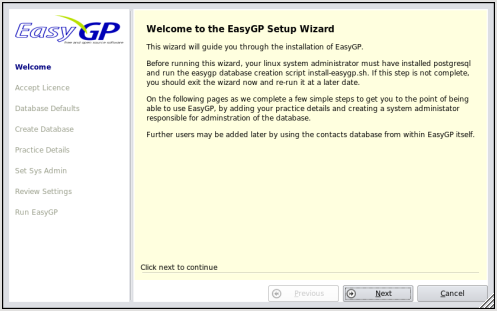
\includegraphics[width=\linewidth]{gettingstarted/setupwizard-page1.png}
\end{minipage}
\hspace{0.5cm}
\begin{minipage}[b]{0.65\linewidth}

\end{minipage}
\end{figure}




There are a number of steps to complete


\begin{itemize}
\item  The Introduction
\item  Accept the licence agreement
\item  Creating your practice organisation
\item  Creating a system administrator
\item  Reviewing your configuration
\item  Save your configuration
\item  Running EasyGP for the first time\end{itemize}




\subsection{ Licence Agreement}
\label{licence-agreement}
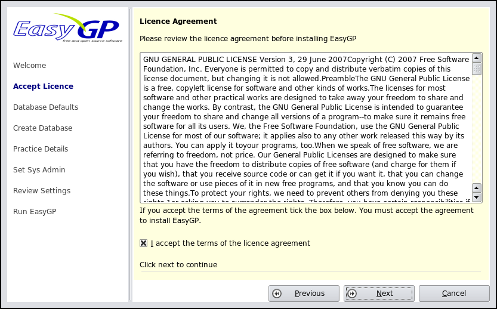
\includegraphics[width=0.8\textwidth]{gettingstarted/setupwizard-page2.png}


You should read the entire text of the licence properly and understand it as you are legally 
obliged to adhere to this licence once you have clicked the accept licence checkupbox and 
installed the software.




\subsection{ Your Practice Details}
\label{your-practice-details}
\begin{figure}[ht] 
\begin{minipage}[b]{0.3\linewidth} 
\centering 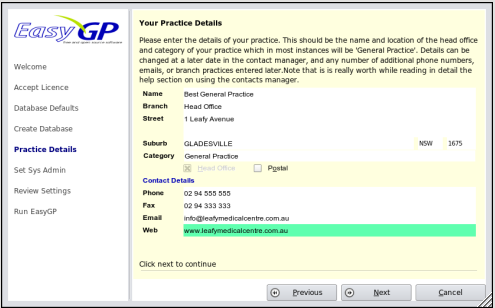
\includegraphics[width=\linewidth]{gettingstarted/setupwizard-page3.png}
\end{minipage}
\hspace{0.5cm}
\begin{minipage}[b]{0.65\linewidth}

\end{minipage}
\end{figure}




In this section you should enter the name of the head office or your organisation
usually this will be the general practice you work in.


The setup wizard will assist you by popping up lists of suburbs, and generally prompting 
you for missing information.


Should you later decided you have made a mistake and have not yet completed the setup
you may use the 'Previous' button to re-visit any of the pages. 


After completion of the setup wizard, this information can of course be changed
in the EasyGP Contacts Manager.


{\bf A Special note about using categories.} 

Categories are used extensively in EasyGP to help you organise your information.Here we mean
the type of category you wish your organisation to belong to - usually a 'general practice'.




\subsection{ The System Administrator}
\label{the-system-administrator}
\begin{figure}[ht] 
\begin{minipage}[b]{0.3\linewidth} 
\centering 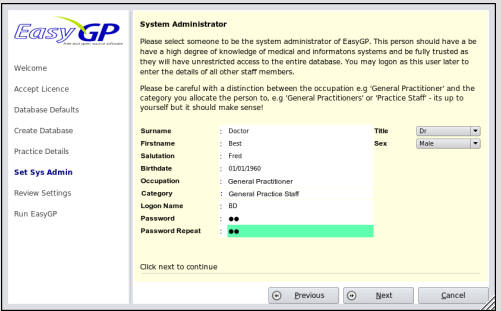
\includegraphics[width=\linewidth]{gettingstarted/setupwizard-page4.png}
\end{minipage}
\hspace{0.5cm}
\begin{minipage}[b]{0.65\linewidth}

\end{minipage}
\end{figure}


The system administrator should be a trusted member of your staff and should have 
a reasonable knowledge of Information Technology and using computer programs as they 
will be given access rights to all modules and database functions.




\subsection{ Previewing your setup}
\label{previewing-your-setup}
\begin{figure}[ht] 
\begin{minipage}[b]{0.3\linewidth} 
\centering 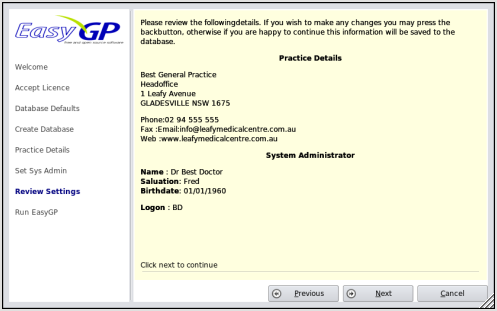
\includegraphics[width=\linewidth]{gettingstarted/setupwizard-page5.png}
\end{minipage}
\hspace{0.5cm}
\begin{minipage}[b]{0.65\linewidth}

\end{minipage}
\end{figure}


You will be presented with a summary of the information you have entered.


This page is the last chance to either go back and change what you are not happy about, or 
to cancel the wizard.
 
Once you click the 'Next' button, the data from the wizard will be written to the database.






\subsection{Completing the initial setup}
\label{completing-the-initial-setup}
\begin{figure}[ht] 
\begin{minipage}[b]{0.3\linewidth} 
\centering 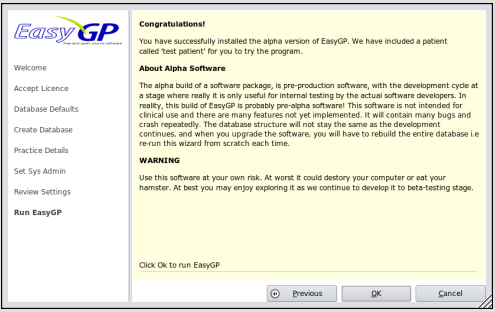
\includegraphics[width=\linewidth]{gettingstarted/setupwizard-page6.png}
\end{minipage}
\hspace{0.5cm}
\begin{minipage}[b]{0.65\linewidth}

\end{minipage}
\end{figure}


At this point you may run easygp, either as the user you entered as sysadmin or as 'easygp' 
the latter of course will not be able to access any clinical records. You may however add more 
staff members, organisations such as hospitals, pathology providers etc,\section{Importing data}
\label{importing-data}
\section{Starting EasyGP}
\label{starting-easygp}


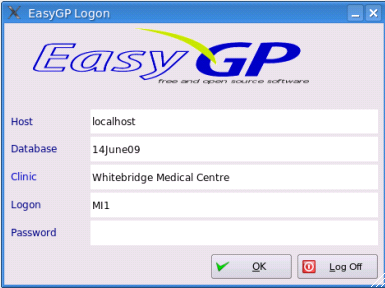
\includegraphics[width=0.8\textwidth]{gettingstarted/logon.png}


When you first run EasyGP you will be presented with the logon screen
\begin{itemize}
\item  Host is the address of the server running an easyGP database, either on the local network or on the Internet. It will usually be set to the default `localhost' (meaning the same computer), but can be a domain name or an IP address.

\item  Database is the name of the database you wish to access, almost always `easygp'.
\item  User is your user code, usually your initials. Remember the easygp administrator user is always `easygp'.
\item  Password is your assigned password. For the admin user this was entered during the install process inBuilding your Database (see page \pageref{building-your-database}). Note this adminstrator user can't access clinical screens: for medico-legal reasons any clinical action taken by a user
must be mappable to a real person. user accounts with real people's names can be created through the Contacts
section (
Contacts (see page \pageref{contacts})) which the administrator does have access to.
\end{itemize}
\section{Closing EasyGP}
\label{closing-easygp}


EasyGP can closed like other graphical application by using the button in the far right corner (the appearance varies from system to system)








\chapter{Basic Concepts}
\label{basic-concepts}


It is vital that before using EasyGP  you learn a little bit about how the program is constructed, and how to use and navigate 
around the graphics user interface (GUI).


{\bf Icon Sets for components} 

It is really important that you understand that your Linux Distribution your choices of its configuration will affect the 
appearance of the icon set within EasyGP, and that the icons used in this help file, my be different from those which you see.


{\bf Configuration File} 

As virtually every screen component in EasyGP is configurable, to run EasyGP you must have the file 'easygp.conf' on your 
computer, otherwise, the GUI could look very strange indeed, as this file contains all the information for the various 'splitters' 
which control the internal geometry and placement of the GUI components.
\section{Focus}
\label{focus}


Gui objects are all those things which make up the screen you are viewing - the labels, textboxes, lists, buttons and so-on. Some objects 
do nothing but sit there for example a label. Others, such as lists have behaviours which allow you to scroll up and down them, and others 
such as textboxes and word processors accept data input which can be later saved by the program.


When you click on, or tab to, or arrive at by any means, an object, for example a textbox - then it 'has focus' - i.e it is the centre 
of attention for the moment. So, how do you know that an object has focus?


{\bf Textboxes} 



\begin{figure}[ht] 
\begin{minipage}[b]{0.3\linewidth} 
\centering 
\includegraphics[width=\linewidth]{basicconcepts/focus_textbox_cursor.png}
\end{minipage}
\hspace{0.5cm}
\begin{minipage}[b]{0.65\linewidth}
\begin{itemize}

\item  Flashing cursor visible in textbox
\end{itemize}

\end{minipage}
\end{figure}


\begin{figure}[ht] 
\begin{minipage}[b]{0.3\linewidth} 
\centering 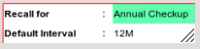
\includegraphics[width=\linewidth]{basicconcepts/focus_txtbox_green.png}
\end{minipage}
\hspace{0.5cm}
\begin{minipage}[b]{0.65\linewidth}
\begin{itemize}

\item  Change of background colour - this will (later) be made configurable in EasyGP
\end{itemize}

\end{minipage}
\end{figure}


\begin{figure}[ht] 
\begin{minipage}[b]{0.3\linewidth} 
\centering 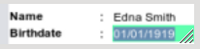
\includegraphics[width=\linewidth]{basicconcepts/focus_textbox_highlighted.png}
\end{minipage}
\hspace{0.5cm}
\begin{minipage}[b]{0.65\linewidth}
\begin{itemize}

\item  change in background colour of the selected text
\end{itemize}

\end{minipage}
\end{figure}


{\bf Buttons} 

\begin{figure}[ht] 
\begin{minipage}[b]{0.3\linewidth} 
\centering 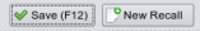
\includegraphics[width=\linewidth]{basicconcepts/focus_buttons.png}
\end{minipage}
\hspace{0.5cm}
\begin{minipage}[b]{0.65\linewidth}
\begin{itemize}

\item  There is usually some sort of dotted outline around buttons which have focus
\end{itemize}

\end{minipage}
\end{figure}


{\bf Lists} \begin{figure}[ht] 
\begin{minipage}[b]{0.3\linewidth} 
\centering 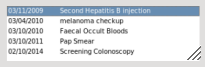
\includegraphics[width=\linewidth]{basicconcepts/focus_listbox.png}
\end{minipage}
\hspace{0.5cm}
\begin{minipage}[b]{0.65\linewidth}
\begin{itemize}

\item  The line selected will be highlighted by a (usually system wide) foreground color or 'marquee'
\end{itemize}

\end{minipage}
\end{figure}


{\bf Change in 3D} 

some controls such as panels and buttons may appear:




\begin{figure}[ht] 
\begin{minipage}[b]{0.3\linewidth} 
\centering 
\includegraphics[width=\linewidth]{basicconcepts/focus_no_3d.png}
\end{minipage}
\hspace{0.5cm}
\begin{minipage}[b]{0.65\linewidth}
\begin{itemize}

\item  Flat when they have no focus
\end{itemize}

\end{minipage}
\end{figure}


\begin{figure}[ht] 
\begin{minipage}[b]{0.3\linewidth} 
\centering 
\includegraphics[width=\linewidth]{basicconcepts/focus_has_3d.png}
\end{minipage}
\hspace{0.5cm}
\begin{minipage}[b]{0.65\linewidth}
\begin{itemize}

\item  Raised and outlined when they have no focus
\end{itemize}

\end{minipage}
\end{figure}
\section{Keyboard Navigation}
\label{keyboard-navigation}


When computers first trickled into general practice in the mid 1990's, I spent some time coaxing, co-ercing, and tutoring doctors in the 
clinical use of computers, and spent many hours sitting side by side with them watching them struggle using the graphics user interface. Sadly 
despite all the modern advances, in my more recent visits to practices, and in watching secretarial staff use computers, it seems that very few 
persons have ever grasped the basics of navigating around a graphic user interface, nor the concept of Focus. They spend a staggering amount of 
time jumping from keyboard to mouse, clicking something, going back to the keyboard, looking for a key, and in general making life for themselves 
very difficult indeed, and probabaly tripling the amount of time they need to undertake a particular task.


When designing EasyGP we are going to great lengths attempting to make data-entry
{\bf **keyboard centric**} i.e, to allow you to seamlessly navigate from textbox, to combobox, to checkbox, to list, to the final Save button which will then allow yet 
another keypress - enter - to complete the data input process. 
 
Of course this is not always possible and to date in many places in the program,  as EasyGP is a pre-alpha - not even a beta program, it is yet to be implemented.
 
\subsubsection{Key usage conventions}
 
These are common by and large to windows and unix/linux systems, with one major exception that in linux there are two copy buffers - 
one filled by just swiping the text (no need to use popup menu or Ctrl C) and they other Ctrl C.


It should be possible to navigate up and down within 
the edit area (see page \pageref{the-edit-area}) using these keys, including from combo-boxes and checkboxes 
Where this is not possible please let us know and I will insert the code.


\begin{itemize}
\item   Enter and Tab  - go down from one control to another
\item  Shift Tab  -go up to the next control\end{itemize}
{\bf Combox box} 

\begin{itemize}
\item  Spacebar - exposes the drop down list
\item  Arrow keys go up and down
\item  Enter key accepts the item\end{itemize}
{\bf Checkbox} 

\begin{itemize}
\item  Spacebar switches on and off
\item  Enter key move to next control, Shift Tab back to previous control\end{itemize}
{\bf Listboxes and Columnviews} 

\begin{itemize}
\item  Arrow keys go up and down
\item  Enter key accepts the current row as the selected data item and moves to the next CTRL.\end{itemize}
{\bf Special key - the Escape Key} 

If you are somewhere you don't want to be, or want to remove a popup for example a form preview from the screen, use ESC.


{\bf ** In summary: you should resist all temptation to grab your mouse, explore the keyboard options first **} \section{Interface Design}
\label{interface-design}


Most of the graphics user interface components (GUI) in virtually all sections, look the same and function the same way 
irregardless of the content of their information or purpose and it cannot be emphasized enough that
{\bf by learning the concept of using one screen you can apply that to  all the others as they will function the same way.} 

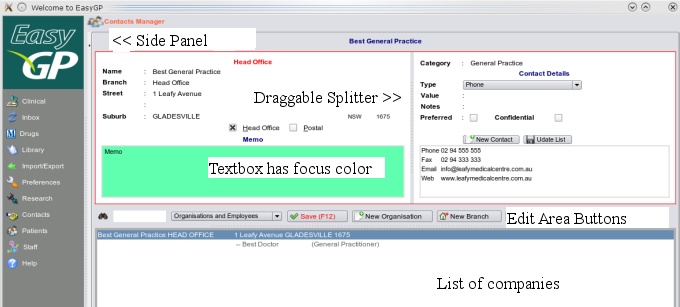
\includegraphics[width=0.8\textwidth]{basicconcepts/gui_features.png}


\begin{itemize}
\item {\bf Side Panels}  - here the almost hidden vertical strip down the left hand side, next to the side bar, when clicked will expand to 
reveal their hidden content, for example this could be a help screen, or a graph. They can be vertical as here, or horizontal as in the 
main clinical screen in the progress notes section. Click these to check out what lies underneath

\item {\bf Splitters}  - These vertical or horizontal serrated lines can be grabbed and moved, and in doing so you will stretch and resize the 
contents, be it textboxes or lists. Adjust these to make the interface as you would like it and use in conjunction with the Application Font.

\item {\bf The Edit Area}  - here enclosed by a red outline indicating data has changed is the most central concept in EasyGP 
and will be discussed ad-nauseum in a later section. Here, new information is entered, or existing information is changed.

\item {\bf Edit Area Buttons}   - usually Save, New, Preview, Print or variations of this will save any changes of data in the Editing area.

\item {\bf Data Lists}  - usually live under the editing area and contain lists of information - e.g names, here of companies, but in other places 
the list will be of patients, medical conditions, vaccinations etc.

\item {\bf PopupMenu's}  - abound everywhere, usually over lists, but can be over panels and let you action items on the list, e.g delete, print, or let you 
   adjust things like font and colour of the list or panel.

\item {\bf Color Changes} - are used extensively to indicate either, as here, a textbox has focus, or as here, data has changed - here the entire editing area which 
has become outlined in red as data changes.
\end{itemize}
{\bf Note}  that any adjustments you make to a screen will be automatically saved when the program exits. If it does not then there is a bug 
in that section and you should notify us immediately.
\subsection{Splitters}
\label{splitters}


As mentioned in the previous section splitters enable the user to re-size area's of the screen and its contents, and there are two 
types:




\begin{figure}[ht] 
\begin{minipage}[b]{0.3\linewidth} 
\centering 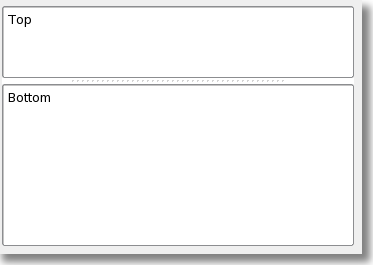
\includegraphics[width=\linewidth]{basicconcepts/vertical_splitter.png}
\end{minipage}
\hspace{0.5cm}
\begin{minipage}[b]{0.65\linewidth}


\begin{itemize}

\item  {\bf A Vertical Splitter }  is a container that lays out its children vertically, and that allows the user to resize them by dragging the boundary between them

\end{itemize}

\end{minipage}
\end{figure}


\begin{figure}[ht] 
\begin{minipage}[b]{0.3\linewidth} 
\centering 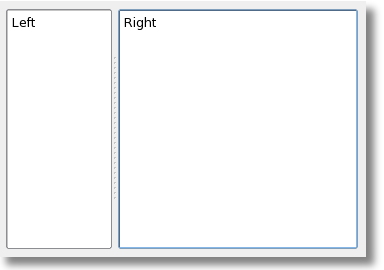
\includegraphics[width=\linewidth]{basicconcepts/horizontal_splitter.png}
\end{minipage}
\hspace{0.5cm}
\begin{minipage}[b]{0.65\linewidth}


\begin{itemize}

\item  {\bf A Horizontal Splitter } is a container that lays out its children horizontally, and that allows the user to resize them by dragging the boundary between them. 

\end{itemize}

\end{minipage}
\end{figure}


EasyGP makes extensive use of splitters and will automatically save your resized screen area's on exit. If you find your self in a
 section of EasyGP and the screen design looks a little odd, its possible you have accidentally moved a splitter right up to the top 
or out to one edge, and hidden its contents - go take a look, grab the line and drag it back.


This help file you are reading now, has a vertical splitter separating the chapters/topics from the text you are reading - try 
adjusting this as practice in using splitters.


 \subsection{Side Panels}
\label{side-panels}


\begin{figure}[ht] 
\begin{minipage}[b]{0.3\linewidth} 
\centering 
\includegraphics[width=\linewidth]{basicconcepts/side_panel.png}
\end{minipage}
\hspace{0.5cm}
\begin{minipage}[b]{0.65\linewidth}


\begin{itemize}

\item  This is a container that can be hidden or resized  and its handles can face sideways, downwards or upwards.\end{itemize}
\begin{itemize}
\item  It is hidden or shown when the user clicks on one of the two small arrow buttons displayed on its border.
\item   It is resized when the users clicks on the border between the buttons, and moves the mouse. \end{itemize}

\end{minipage}
\end{figure}




\begin{figure}[ht] 
\begin{minipage}[b]{0.3\linewidth} 
\centering 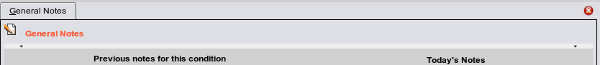
\includegraphics[width=\linewidth]{basicconcepts/side_panel_closed.png}
\end{minipage}
\hspace{0.5cm}
\begin{minipage}[b]{0.65\linewidth}
\begin{itemize}

\item  As an example in the main clinical window here is a closed side panel, oriented towards the top - notice the little arrows:\end{itemize}

\end{minipage}
\end{figure}
. 
. 
. 
\begin{figure}[ht] 
\begin{minipage}[b]{0.3\linewidth} 
\centering 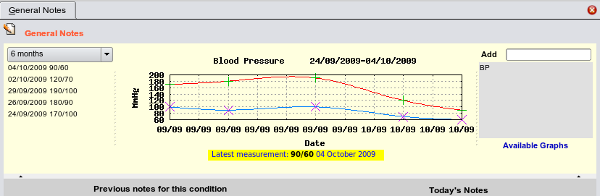
\includegraphics[width=\linewidth]{basicconcepts/side_panel_open.png}
\end{minipage}
\hspace{0.5cm}
\begin{minipage}[b]{0.65\linewidth}


\begin{itemize}

\item  Surprise surprise - it hides a wealth of information - in this case a configurable measurements panel - here just showing BP's:\end{itemize}

\end{minipage}
\end{figure}


Other sections of the program make use of vertical side panels which hide for example decision support or help.\subsection{The Edit Area}
\label{the-edit-area}


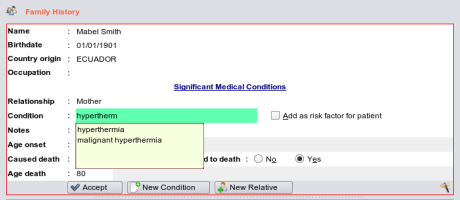
\includegraphics[width=0.8\textwidth]{basicconcepts/sample_editarea.png}


Please note - this is 
{\bf the most important part of the entire help file } 

You should read this until you fully understand it. Using the editing area's effectively 
will save you buckets of time and learning to use the keyboard will mean 
{\bf  **you  very rarely have to use the mouse***.} 

{\bf Edit Area Principals} \begin{itemize}
\item {\bf Add New is the Default State } of an editing area  i.e it is to be ready to accept new data. When a section first loads, or after a save, the next action 
expected of the user is that he will want to add more data. Clearing the editing area, by using a 'Clear' or 'New..' button 
also re-sets the editing area to its expectant state.

\item {\bf Concept of Focus} - Whatever is the area of the screen being used for data entry it 'has focus' and in EasyGP if this is a textbox then focus will 
be indicated by a  green backcolor(configurable), or, if a drop down combo box or button, by some visible black outlining of
the control.

\item {\bf Popup Lists}  - will be presented where information exists to assist you in auto-completing data, use the down arrow key to scroll to the list not the mouse 
 and the enter key to accept the data.

\item {\bf Data is Validated } prior to save and you will be prompted for any missing data but not all data entry fields are mandatory.

\item {\bf Save (F12)} immediately saves the data to the database backend and any relevant list underneath the editing area refreshed.

\item {\bf EditArea's can be Partially cleared} for example adding multiple conditions to the one family member.

\item {\bf Editing area's within an Edit area} can exist, for example in the contacts database and operate in principal the same as their parent except internal lists are not
saved until the entire editing area content is saved via the Save button.

\item {\bf Editing existing information in the lists } is done by either clicking on the item in the list, which in some sections will automatically load the data back into the editing area 
as an implicit edit, or by right mouse clicking on the list and selecting 'Edit'.

\item {\bf Auxillary data entry area's} may exist within an editing area such as a word processor in say a letter writer.

\item {\bf Data is Deleted} by seleting the data item from the list underneath the editing area and selecting Delete from the popup menu.

\item {\bf GUI elements } such as textboxes and lists are adjustable by grabbing the horizontal and vertical sliders and shutdown will save this automatically.

\item {\bf Your actions will be audited } - no matter what you do, an audit trail is kept of everything you add and delete or alter and you may be asked for an explanation. 
\end{itemize}
{\bf Key Usage Defaults} \begin{itemize}

\item {\bf ENTER or TAB }  will move the focus to the next control in the tab order, be it textbox or combobox etc and implicitly accepts the data 
in the textbox or combobox or checkbox. Hitting enter in a textbox will move you to the next one (although some may be 
skipped if they are rarely used) right up to the Save button.

\item {\bf DOWN ARROW}  from a textbox will move the cursor onto a popup list if the list is visible

\item {\bf SPACEBAR}   when a combobox has focus will drop down the list for that combo, or if a checkbox will check or uncheck the box
\end{itemize}
\subsection{Column Widths for Lists}
\label{column-widths-for-lists}


Wherever there are lists with multiple columns, it's a fair bet that the content of each column will not visually suit many 
computer monitor resolutions, so on the popup menu overlying these lists, there is usually an option to adjust the column widths, 
which are then saved back to a configuration file once the form is closed or the program exits.


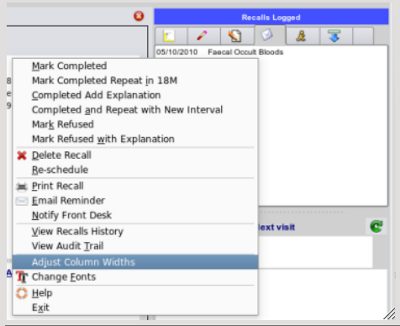
\includegraphics[width=0.8\textwidth]{basicconcepts/adjust_columnwidths_menu.png}


Once you have clicked on the 'Adjust Column widths' option on the menu, an adjustable column header will appear over the list. 




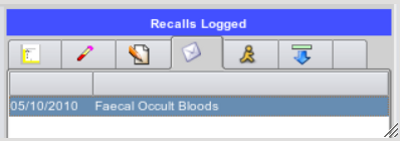
\includegraphics[width=0.8\textwidth]{basicconcepts/adjust_columnwidths_header.png}




You may grab the little divider with the mouse and adjust the size of all the columns.


Once satisfied with the visual appearance, just click on any row in the list and the adjustments will be saved.


\subsection{Fonts}
\label{fonts}


There are a number of mechanisms to adjust the fonts throughout the program, system wide application font, and fonts on 
individual controls


\subsubsection{Application Font}


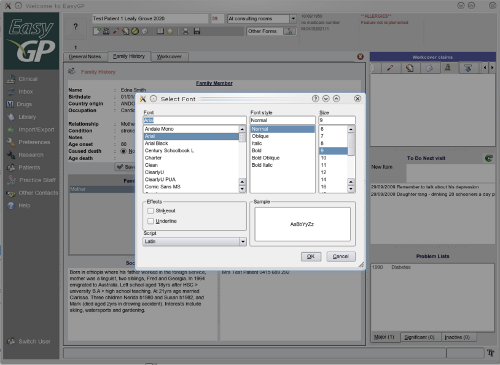
\includegraphics[width=0.8\textwidth]{basicconcepts/application_font.png}




You may change the font and font size for the entire application by clicking on the little 
font button, 



\includegraphics[width=0.8\textwidth]{basicconcepts/font_button.png}


 located on the lower right hand side of the screen status bar. This setting is immediately applied. 


\subsubsection{Fonts for Lists}
 
 In many sections of the program, on the popup menu that you may view by right mouse clicking on 
 the lists, there is an option to change the font for that list. This over-rides any system wide 
 font changes.
 


 
\subsubsection{Browser font sizes}


Browser windows are used extensively in EasyGP, for example to view progress notes, care plans, reports etc, and as the browser 
contains html, you must zoom up and down to adjust the font sizes as you would in a normal internet browser.


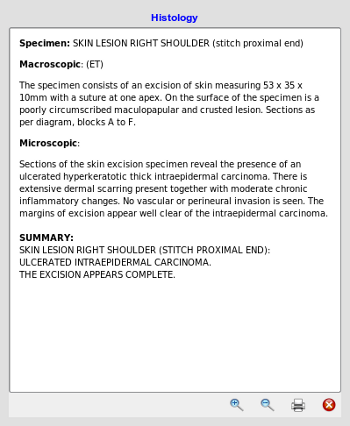
\includegraphics[width=0.8\textwidth]{basicconcepts/adjust_fonts_browsers.png}


Each browser window has icons to expand or shrink the font for that window. 



\includegraphics[width=0.8\textwidth]{basicconcepts/adjust_fonts_browsers_zoom_in.png}
  makes the font size large



\includegraphics[width=0.8\textwidth]{basicconcepts/adjust_fonts_browsers_zoom_out.png}
  makes the font size smaller.


The new zoom size will be saved when either its screen is closed, or the application exits.

 


 
\section{Auditing}
\label{auditing}


Every time data is written to the database in EasyGP it is in some way audited, though most this occurs 'under the hood', and will not be 
intrusive to the user.


Where information is being changed from that which currently exists in the database - either when a record is being in some way changed or 
deleted, then the auditing will enforce the rule that the user enter a reason for why this is occuring 
{\bf unless explicitly stated otherwise. } For example a popup menu may have an option to undertake an action such as "Mark complete with no explanation", in which case, the user, 
by accepting this option, is taking responsiblity for this action.


For example in the scratchpad section, when you delete an item, ie it was not actioned as completed in some way, but is being removed, 
then you will have to complete this dialog:




\begin{figure}[ht] 
\begin{minipage}[b]{0.3\linewidth} 
\centering 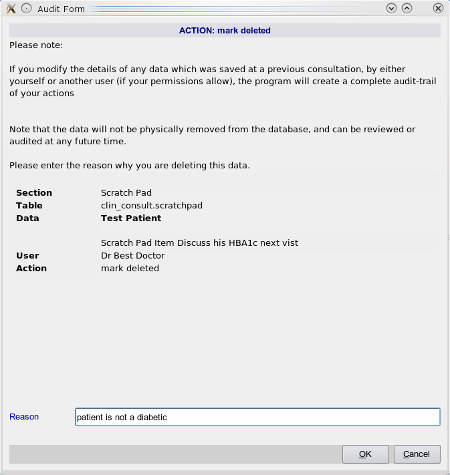
\includegraphics[width=\linewidth]{basicconcepts/scratchpad_audit_delete.png}
\end{minipage}
\hspace{0.5cm}
\begin{minipage}[b]{0.65\linewidth}
\begin{itemize}

\item  The following information will always be supplied:\end{itemize}
\begin{itemize}
\item  The current user who is undertaking the action - yourself
\item  The patient's name
\item  The type of action eg Deletion
\item  The data being changed or deleted\end{itemize}
\begin{itemize}

\item \end{itemize}
\begin{itemize}

\item \end{itemize}
\begin{itemize}

\item \end{itemize}
\begin{itemize}

\item  The Reason for the action must then be supplied by the user, or the action cancelled.\end{itemize}

\end{minipage}
\end{figure}


As an example of reviewing audited data please see the help section for the scratch pad 
Scratch Pad Audit (see page \pageref{scratch-pad-audit})

{\bf Note: } 

This audit trail including data time hour and minute will always be available for medico-legal reasons and can never be changed.


\section{Permissions}
\label{permissions}




\section{Selecting Program Sections}
\label{selecting-program-sections}


\begin{figure}[ht] 
\begin{minipage}[b]{0.3\linewidth} 
\centering 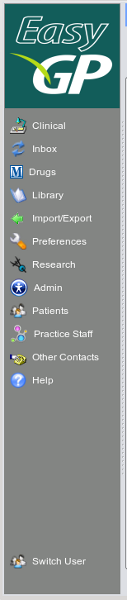
\includegraphics[width=\linewidth]{basicconcepts/selecting_sections.png}
\end{minipage}
\hspace{0.5cm}
\begin{minipage}[b]{0.65\linewidth}


\begin{itemize}

\item  {\bf Accessing Sections of the Program} \end{itemize}
\begin{itemize}

\item  The side bar is similar to the 'Outlook' style panel that everyone has become very familiar with 
and each of the buttons on the side bar will open a section of the program.
\end{itemize}
\begin{itemize}

\item Clinical (see page \pageref{clinical})- All patient specific clinical information will be entered or viewed in this section.
  It will allow you to enter family history, past history, occupational history, 
  mental health issues, skin proceedures, workers compensation, full progress notes, forms for every
  conceivable thing you could order, travel medicine, care planning, just to mention a few. 

\item Inbox (see page \pageref{inbox})- This section contains all incoming information for patients (plural), be it electronic pathology results,
   radiology reports, letters from specialists, emails, scanned documents or hospital discharge summaries. From here
   you may file and action any document, including insert progress notes or recalls into the patients notes.

\item Drugs (see page \pageref{drugs})- Look up full drug product information.

\item Library (see page \pageref{library})- keep all your favourite references and handouts.

\item Research (see page \pageref{research})- A tool to explore your clinical data.

\item Import/Export (see page \pageref{import/export})- Import data in and out of EasyGP.

\item Admin (see page \pageref{admin})- Manage administrative tasks such as the recall system.

\item Patients (see page \pageref{patients})- manage your patients database

\item Practice Staff (see page \pageref{practice-staff})- manager the staff in your practice, their names, addresses, preferences and logon information and passwords.

\item Other Contacts (see page \pageref{other-contacts})- all organisations, their branches and employees are entered here.

\end{itemize}

\end{minipage}
\end{figure}
\chapter{Contacts Manager}
\label{contacts-manager}


{\bf Note: } Your icon set will be determined by your linux window manager settings, so icons used in these illustrations will 
almost certainly differ from the ones you see on the screen.


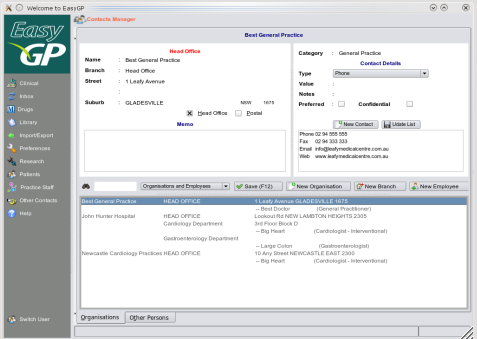
\includegraphics[width=0.8\textwidth]{contacts/othercontacts/organisations/organisations_listing.png}


This is probably
{\bf the most} important module in the whole of the program and it is absolutely essential that you take the time
to read and understand its functioning in detail before building and running your program. 




The contacts database is central to the functioning of EasyGP. 


It contains


\begin{itemize}
\item  Patient information and demographic details
\item  Organisations, their branches and their employees which includes your staff
\item  All persons not in the above two categories\end{itemize}
To aid in keeping information in a logical manner, it is functionally split up into three sections within 
the graphics user interface accessable via the
the side bar (see page \pageref{the-side-bar}):


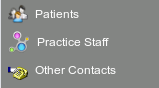
\includegraphics[width=0.8\textwidth]{contacts/general/contacts_three_sections.png}


Whereas EasyGP will function adequately if you edit the data any-old-how, to get the most out 
of the program it is vital to structure your contacts data logically.
\section{Allocating Categories}
\label{allocating-categories}


{\bf What is a category and what are they for?} 

{\bf n. pl. categories: A specifically defined division in a system of classification or a class.} 

We use categories to organise information and when you enter any data in the contacts manager, one of the 
obligatory fields is it's 'category'. As you will later use these categories to retrieve information you 
should make every effort to be use ones that make sense.


As examples, in the patients module - all persons enterered automatically belong to the 'patients' category. 
In the Organisations module, public hospitals should be allocated to a 'Public Hospital' category, and so on. A person 
in the 'patient' category could be allocated  to the 'Radiographer' category in the Organisations Module if they happen 
to work in the local radiology firm and are also your patient.


As you type in the categories text box the following will appear: Here we have typed a single letter 'p' to 
obtain the list. 


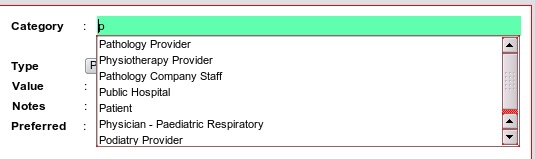
\includegraphics[width=0.8\textwidth]{contacts/general/contacts_allocating_categories.png}


Once you can see the category you want use the down arrow key on the keyboard to scroll down to the item you 
want, and then hit the $<$enter$>$ key. Resist all tempation to take your hands off the keyboard and use the mouse!


Some basic categories are supplied, however there are an infinite number of categories  so of course you can add 
your own, and they will be automatically  saved for future use.


\begin{figure}[ht] 
\begin{minipage}[b]{0.3\linewidth} 
\centering 
\includegraphics[width=\linewidth]{common/graphics/ktip.png}
\end{minipage}
\hspace{0.5cm}
\begin{minipage}[b]{0.65\linewidth}


Typing in the wildcard character (\%) in any textbox in EasgGP will give a complete list of results (e.g all the categories) which 
could be quite large, so take care with this.

\end{minipage}
\end{figure}


{\bf Special Category - The Provider} 

There is only one special category in EasyGP and it is that of a 'Provider'.


{\bf A Provider is defined as an entity - be it an organisation or a person - who supplies services to your practice. } 

Most of the clinical sections use this concept to retrieve 
information for you .For example if you allocate your pathology companies to 'Pathology Provider', then you will have automatic access to 
their details, Similarly for 'Cardiology Provider' or 'Physiotherapy Provider', and you can even make up your own categories 
or providers.  Then within the Requests ordering section you will be able to order tests linked to that provider type.


\section{Add Contact Method}
\label{add-contact-method}


We use the term 'contact method' or 'communication' in the broadest sense. Gone are the days when a persons 'home phone' was a fixed land line. 
This century it is more likely to be a mobile phone, VOIP etc, rather than a fixed line. Hence a 'communication' is any method 
of contacting a person.


{\bf Adding a New Contact Method} 

\begin{figure}[ht] 
\begin{minipage}[b]{0.3\linewidth} 
\centering 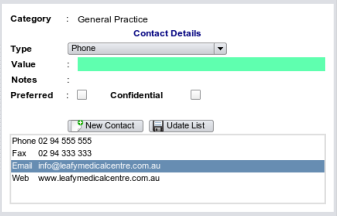
\includegraphics[width=\linewidth]{contacts/general/contacts_new_contact_button.png}
\end{minipage}
\hspace{0.5cm}
\begin{minipage}[b]{0.65\linewidth}


\begin{itemize}

\item  Clicking the add new button within the editing area will clear any text in the contact details area, the cursor will appear in the 'value' textbox.
\end{itemize}
\begin{itemize}

\item  Here you should enter the details such as the phone number, web address etc.\end{itemize}

\end{minipage}
\end{figure}






\begin{figure}[ht] 
\begin{minipage}[b]{0.3\linewidth} 
\centering 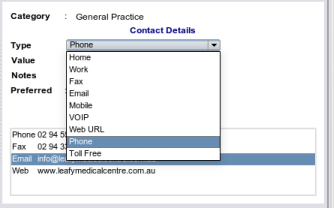
\includegraphics[width=\linewidth]{contacts/general/contacts_new_contact_type.png}
\end{minipage}
\hspace{0.5cm}
\begin{minipage}[b]{0.65\linewidth}


\begin{itemize}

\item   As there is a small amount of intelligence built in, EasyGP will recognise if the text represents a mobile phone, web address or email address and set the  type combo box accordingly.
\end{itemize}
\begin{itemize}

\item  If this cannot happen automatically e.g it is a home phone, then it is important you set the type accurately, and clicking the type combo-box will give you a complete list of options.

\end{itemize}

\end{minipage}
\end{figure}






\begin{figure}[ht] 
\begin{minipage}[b]{0.3\linewidth} 
\centering 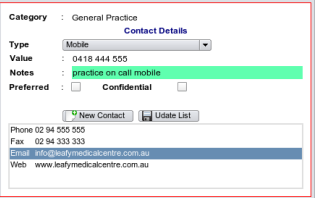
\includegraphics[width=\linewidth]{contacts/general/contacts_new_contact_data.png}
\end{minipage}
\hspace{0.5cm}
\begin{minipage}[b]{0.65\linewidth}




\begin{itemize}

\item  Notes - add any qualifying information about the contact method \end{itemize}
\begin{itemize}

\item  Preferred checkbox - if checked, then this will be the preferred way to communicate with the person/employee/organisation\end{itemize}
\begin{itemize}

\item  Confidential checkbox- the communication will be treated as confidential \end{itemize}

\end{minipage}
\end{figure}


clicking the Update button will add the new information to the list.


Note that this
{\bf has not } saved the new phone numbers to the database. When you wish to save a new or modified entry, you must click on the main 
Save button, as shown here:


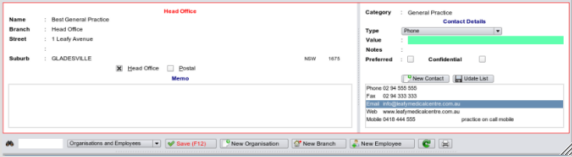
\includegraphics[width=0.8\textwidth]{contacts/general/contacts_new_contact_save.png}


{\bf Editing or Deleting and Existing Contract} 

Clicking on the list of existing contacts will give you a popup menu to allow editing (changing) or deleting, the highlighted 
contact. You must of course remember to save your data after any editing.
\section{Adding Addresses}
\label{adding-addresses}


The EasyGP database structure allows a 'one to many' relationship between Organisations, persons and addresses. Translated into 
plain english this means that a person can have none, one, or many addresses, and the same for Organisations, however the way 
this is handled differs between persons and organisations. 


{\bf Adding an Address to an Organisation.} 

The mechanics of this are identical to adding addresses for a person except for one factor. As an organisation has one or many 
branches technically each branch only has a single address so there is no 'list' of addresses for organisations within the edit area.


{\bf Content of the Address Fields} 

As the term 'address' is used in a loose way it could be:
\begin{itemize}
\item  An actual street complete with suburb
\item  A street with no suburb
\item  A suburb with no street
\item  The location of a  department e.g 3rd Floor Block D, with no other information if it is a branch address
\item  Can be the 'default address' or a 'postal address'.\end{itemize}
{\bf Adding Addresses to Patients or other People} 

\begin{figure}[ht] 
\begin{minipage}[b]{0.3\linewidth} 
\centering 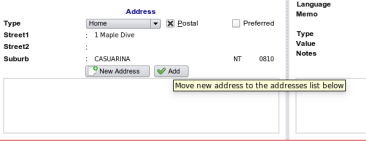
\includegraphics[width=\linewidth]{contacts/general/address_new_enter_data.png}
\end{minipage}
\hspace{0.5cm}
\begin{minipage}[b]{0.65\linewidth}


\begin{itemize}

\item  As described in the section on adding phone numbers, just enter the street and suburb details or whatever minimum amount of
information is required. Note that in some sections you will be prompted at the time you save the record if anything is missing.
\end{itemize}
\begin{itemize}

\item Australian suburbs and postcodes are supplied with EasyGP and will appear automatically as you type. A valid town must be 
selected and free text is not allowed.

\end{itemize}

\end{minipage}
\end{figure}


\begin{figure}[ht] 
\begin{minipage}[b]{0.3\linewidth} 
\centering 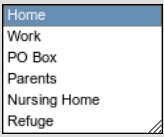
\includegraphics[width=\linewidth]{contacts/general/address_types.png}
\end{minipage}
\hspace{0.5cm}
\begin{minipage}[b]{0.65\linewidth}
\begin{itemize}

\item Whilst most addresses in the patients section will be home addresses (the default), you have the option of a number of others
 by clicking the drop down combobox.
\end{itemize}

\end{minipage}
\end{figure}


Once happy with the data, click the 'Add' button and the address will appear on the list below the address data entry area. 
Remember that this data is not saved to the database until the Save button is clicked (or F12 key pressed).


{\bf Editing or Deleting an Existing Address} 

Clicking the right mouse button will give you the options of editing (to allow change) or deleting an existing address.
\section{Adding a Photograph}
\label{adding-a-photograph}




In many sections of EasyGP including the contacts modules for patients and staff, it is possible add a photo to 
the database. The screen images  here are the same for both these sections named above.


By default no image exists and a placeholder will always be shown.


\begin{figure}[ht] 
\begin{minipage}[b]{0.3\linewidth} 
\centering 
\includegraphics[width=\linewidth]{contacts/patients/patients_new_photo_empty.png}
\end{minipage}
\hspace{0.5cm}
\begin{minipage}[b]{0.65\linewidth}
\begin{itemize}

\item \end{itemize}


\begin{itemize}

\item {\bf Aquire  } This feature is not yet implemented
\end{itemize}
\begin{itemize}

\item {\bf Remove} If you have previously loaded a patient's photo and wish to remove it the photo picturebox will be reset.

\end{itemize}

\end{minipage}
\end{figure}


\begin{figure}[ht] 
\begin{minipage}[b]{0.3\linewidth} 
\centering 
\includegraphics[width=\linewidth]{contacts/patients/patients_new_photo_loaded.png}
\end{minipage}
\hspace{0.5cm}
\begin{minipage}[b]{0.65\linewidth}
\begin{itemize}

\item {\bf Load  } Clicking this will present you with a file dialog to load an existing photograph
\end{itemize}

\end{minipage}
\end{figure}


Note as with all information within an editing area, it will not be saved until the Save Button (F12) is clicked in the relevant section. 


\section{Patients}
\label{patients}




\includegraphics[width=0.8\textwidth]{contacts/patients/patients_main.png}


The patients module is used to add new patients to EasyGP.


Should you wish to import patients from another medical records program, please see the section 
Importing Patients (see page \pageref{importing-patients}) 


\subsection{Patient Demographic Details}
\label{patient-demographic-details}


Most of this is straightforward. You will be prompted with lists of surnames and firstnames if they exist.


\begin{figure}[ht] 
\begin{minipage}[b]{0.3\linewidth} 
\centering \includegraphics[width=\linewidth]{contacts/patients/patients_firstname_surname.png}
\end{minipage}
\hspace{0.5cm}
\begin{minipage}[b]{0.65\linewidth}


\begin{itemize}

\item {\bf birthdate} This needs to be entered either as dd/mm/yyy or any similar combination eg 9/9/53 or 09/9/1953. If the program cannot 
convert your input to a date you will be re-prompted until the data is valid
\end{itemize}
\begin{itemize}

\item {\bf Salutation} It is surprising how many people do not know this term - it means how the person likes to be addressed for example 
sometimes a person may have disliked their firstname e.g Gladys and has always used their middle name e.g Kathryn, so 
the salutation field would be Kathryn.

\end{itemize}

\end{minipage}
\end{figure}


{\bf Address(s)}     see  
Adding Addresses (see page \pageref{adding-addresses})

{\bf Contact Numbers}     see  
Add Contact Method (see page \pageref{add-contact-method})

{\bf Patient Photo}     see
Adding a Photograph (see page \pageref{adding-a-photograph})

{\bf Ethnicity} \begin{figure}[ht] 
\begin{minipage}[b]{0.3\linewidth} 
\centering \includegraphics[width=\linewidth]{contacts/patients/patients_ethnicity.png}
\end{minipage}
\hspace{0.5cm}
\begin{minipage}[b]{0.65\linewidth}
\begin{itemize}

\item {\bf Country}   Refers to the country the patient was born - ie country of origin
\end{itemize}

\end{minipage}
\end{figure}


{\bf The patient Toolbar} 

\includegraphics[width=0.8\textwidth]{contacts/patients/patients_toolbar.png}


\begin{itemize}
\item  Save(F12)     - saves the current data in the editing area
\item  New Patient   - clears the editing area to allow entry of new patient
\item  FamilyMember  - clears the editing area leaving skeletal family data eg address/home phone
\item  Reset  \includegraphics[width=0.8\textwidth]{contacts/patients/contacts_patients_reset_button.png}
  Clears the editing area and the lists.
\subsection{Finding Patients}
\label{finding-patients}
\end{itemize}
There are two options when searching for patients


{\bf Display All Patients } 

\includegraphics[width=0.8\textwidth]{contacts/patients/contacts_patients_search_findall_icon.png}


By clicking on the little search icon a list of all patients will appear in the patients list box. This is  
{\bf not recommended } as your database could have many thousands of patients. This is equivalent to typing the wildcard character 
'\%' in the search textbox (which is also shown above in the picture).


{\bf Selecting patients by pre-defined criteria} 

\includegraphics[width=0.8\textwidth]{contacts/patients/contacts_patients_search_textbox.png}


There are a number of inbuilt queries mechanisms you can type into the patients search box, which is the little 
textbox to the right of the binocular icon shown above.  


\begin{itemize}
\item {\bf Surname,Firstname  } \end{itemize}
\begin{itemize}

\item 'j smit' gives a list of all patients with  firstname starting with 'j' and surname with 'smit'
\end{itemize}
\begin{itemize}
\item {\bf Surname only } \end{itemize}
\begin{itemize}

\item 'smith,' gives a list of all patients with surnames  = 'smith'
\end{itemize}
\begin{itemize}
\item {\bf Firstname only } \end{itemize}
\begin{itemize}

\item 'peter'  gives a list of all patients with firstnames = 'peter'
\end{itemize}
\begin{itemize}
\item {\bf Surname, [Firstname] [sex] [age = $<$ $>$ [between]} \end{itemize}
\begin{itemize}

\item  'peter, age$>$50' gives a list of all patients with firstname peter, age over 50yrs
 
\begin{itemize}

\item 'mary'  s=f age between 40-50 gives all 'mary's' aged between 40 and 50
\end{itemize}
If these fail to work please let us know as though the code is in place they may not yet be 'hooked up'.
\subsection{Importing Patients}
\label{importing-patients}


At some point EasyGP will be able to import most demographic data formats. If your patient database is not supported 
plase contact the developers. The import section is accessed from the Admin button on the side bar.


{\bf Select Program Source } 

\includegraphics[width=0.8\textwidth]{contacts/patients/contacts_patients_import_select_program.png}


{\bf Select Program Version } 

that you are importing from. A popup dialog will appear, you should navigate 
to where your text-delimited data file is, select and select the file.


\includegraphics[width=0.8\textwidth]{contacts/patients/contacts_patients_import_select_datafile.png}


{\bf Type of Import} 

\includegraphics[width=0.8\textwidth]{contacts/patients/contacts_patients_import_select_import_type.png}


\begin{itemize}
\item  Rebuild - will erase any existing patients in the database. This is not possible once the database is being used for clinical purposes

\item  Update  - will attempt to update addresses for existing patients. There may be situations where a person has changed their name or a birthdate was incorrectly input from the original database and has since been corrected. EasyGP 
will attempt to take these possibilities into account and prompt you where ambiguities arise.

\item  Add New since last update - will add only those patients not already present in the database.\end{itemize}
{\bf Data Verification Process} 

If everything is satisfactory, click the 'import button'. EasyGP will perform some basic analysis of your data
\begin{itemize}
\item  Town/Suburb spell checking - for example it will attempt to replace mis-typed names
\item  Postcode check - with insertion of correct or missing postcodes
\item  Firstname/Sex check - with insertion of sex
\item  Title check if possible, defaulting to Ms or Mr for ages $>$ 18 where marital status obviously cannot be deduced\end{itemize}
Any errors will be listed below the import error.


Once completed you may have to go back to the source database and correct any errors. Once happy click the import button.
\subsection{Exporting Patients}
\label{exporting-patients}


This feature is not yet implemented


\section{Practice Staff}
\label{practice-staff}


\includegraphics[width=0.8\textwidth]{contacts/staff/contacts_staff_overview.png}


The staff section is where you enter details of staff members. Note you must logon either as user 'easygp' or have sysadmin rights 
to be able to access this section.


When you installed EasyGP you were prompted to enter the details of your practice which then became then 
default Head Office. Should you have a number of branch offices in your organisation, you should enter those using 
the 'Other Contacts' module which contains information about organisations (such as your own). These branches will then 
be available within the staff module.


The staff module contains sections to allow you to
\begin{itemize}
\item  Add and modify staff members, their names, addresses and contact numbers
\item  Add staff photograph
\item  Record place of work within your organisation
\item  Allocate a security access level, logon code and password
\item  Set up preferences for other sections of EasyGP (feature not implemented)\end{itemize}
\subsection{Staff Demographic Details}
\label{staff-demographic-details}




Most of this is straightforward. You will be prompted with lists of surnames and firstnames if they exist.


\begin{figure}[ht] 
\begin{minipage}[b]{0.3\linewidth} 
\centering \includegraphics[width=\linewidth]{contacts/staff/contacts_staff_staff_details.png}
\end{minipage}
\hspace{0.5cm}
\begin{minipage}[b]{0.65\linewidth}


\begin{itemize}

\item {\bf birthdate} This needs to be entered either as dd/mm/yyy or any similar combination eg 9/9/53 or 09/9/1953. If the program cannot 
convert your input to a date you will be re-prompted until the data is valid
\end{itemize}
\begin{itemize}

\item {\bf Salutation} It is surprising how many people do not know this term - it means how the person likes to be addressed for example 
sometimes a person may have disliked their firstname e.g Gladys and has always used their middle name e.g Kathryn, so 
the salutation field would be Kathryn.

\end{itemize}

\end{minipage}
\end{figure}


{\bf A Special note on Occupation vs Categories} 

Please re-read in the general section on contacts about 
Allocating Categories (see page \pageref{allocating-categories}). It can be pretty easy to confuse data like 'occupation' and 'category'. Take a look at the image above. The doctor's 
occupation is 'General Practitioner', but the category given is 'General Practice Staff'. You could (and of course the 
decision is your own as to how you wish to aggregate information) allocate the person to a category 'General Practitioners' etc. 
Mis-typing something here could make searching for data at a later stage more difficult, so decide your categories carefully. You 
may of course go back at any stage and change any of the information.


{\bf Address(s)}     see  
Adding Addresses (see page \pageref{adding-addresses})

{\bf Contact Numbers}     see  
Add Contact Method (see page \pageref{add-contact-method})

{\bf Staff Photo}     see
Adding a Photograph (see page \pageref{adding-a-photograph})

\subsection{Selecting a Workplace}
\label{selecting-a-workplace}


{\bf Work status } 

The employee's work status is selected from the drop down combo list and can be


\begin{itemize}
\item  Active
\item  On Leave
\item  Departed Organisation
\item  Locum\end{itemize}
\includegraphics[width=0.8\textwidth]{contacts/staff/contacts_staff_work_status_photo.png}








{\bf Place of work } 

The employee's place of work always defaults to head office. 


You may select any of the branches of the organisation 
from the drop down combobox to change this to any branch. Remember that you will have to add new branches to your 
organisation using the 'Other Contacts' module which you can select from the main sidebar buttons.


\includegraphics[width=0.8\textwidth]{contacts/staff/contacts_staff_place_of_work.png}






\subsection{Logon and Security}
\label{logon-and-security}


{\bf Permissions} 

EasyGP permissions are set according to the category's shown in the dropdown combobox list shown above. 
You should select the type of category you wish your staff member to belong to - the permissions for that group will appear 
in the text area underneath the combo box.


\includegraphics[width=0.8\textwidth]{contacts/staff/contacts_staff_logon_security_categories.png}






{\bf Logon Details} 



\begin{itemize}
\item {\bf Logon Name } should be chosen by the user. You will be prompted if duplicate logon names exist

\item  {\bf Validity Dates } can be set from (Now) to an expirey date if desired though this may be left blank (indefinate).

\item {\bf Password } must be repeated.
\end{itemize}
After finished, click the Save button or hit the F12 key.


\includegraphics[width=0.8\textwidth]{contacts/staff/contacts_staff_logon_password.png}






\subsection{Preferences - Providers}
\label{preferences---providers}


Access via the side bar menu $>$ Practice Staff $>$ Doctors Preferences Tab then select the staff member for whom you wish to set 
the preferences.


\includegraphics[width=0.8\textwidth]{contacts/staff/contacts_staff_preferences_providers.png}


Each staff member may individually set preferences for the provider they want EasyGP to use as the default in sections 
such as Request ordering. Doing this will mean that when typing in a request for say a FBC, the pathology company that you 
wish to use and the branch you wish the patient to attend will automatically appear on the request form. Please read the 
Allocating Categories  (see page \pageref{allocating-categories})section for more information on the concept of 'Providers'. 
The companies and branches must of course exist in the contacts database first (see 
Other Contacts (see page \pageref{other-contacts})), however you will be prompted should you try and enter data that does not yet exist.


\begin{figure}[ht] 
\begin{minipage}[b]{0.3\linewidth} 
\centering \includegraphics[width=\linewidth]{contacts/staff/contacts_staff_preferences_completed.png}
\end{minipage}
\hspace{0.5cm}
\begin{minipage}[b]{0.65\linewidth}


\begin{itemize}

\item  {\bf Adding a default provider } \end{itemize}
\begin{itemize}

\item  Click the New Default Provider button, and the select the provider type. If any providers exist they will be presented as a pick list for your choice together with the default head office branch. Complete each line then click the save button (F12).
\end{itemize}

\end{minipage}
\end{figure}






\begin{figure}[ht] 
\begin{minipage}[b]{0.3\linewidth} 
\centering \includegraphics[width=\linewidth]{contacts/staff/contacts_staff_preferences_change_branch.png}
\end{minipage}
\hspace{0.5cm}
\begin{minipage}[b]{0.65\linewidth}


\begin{itemize}

\item  {\bf Changing the default branch.} \end{itemize}
\begin{itemize}

\item  Should you wish a different branch to head office to be the default, click on the branch line and a list of alternate branches for the company will appear (of course you must have entered these in the contacts database!
\end{itemize}

\end{minipage}
\end{figure}
\section{Other Contacts}
\label{other-contacts}


As previously mentioned, in EasyGP, although all the actual data is kept in the same tables within the database, for the purposes 
of data entry, there is a functional separation of contact information into three sections - 
Patients  (see page \pageref{patients}), 
Practice Staff (see page \pageref{practice-staff}), and 
Other Contacts


Other contacts are considered to be
\begin{itemize}
\item  Organisations and their employees, and this includes your own general practice, although you must enter staff specific details such as logon names, security levels etc. within the staff module, as these are specific to your organisation alone.

\item  Persons  not employed by an organisation, for example a 'lone practitioner' or 'specialist' who may have their own rooms but are not part of a company per se.
\end{itemize}
\includegraphics[width=0.8\textwidth]{contacts/othercontacts/othercontacts_tabs.png}


You can select either section from the tab at the bottom of this screen.


\subsection{Organisations}
\label{organisations}


{\bf What is an organisation?} 

There are dozens and dozens of definitions for an organisation!


EasyGP defines organisation is any entity organised for a common purpose, usually considered to be a profit or not for profit 
business or group, under a common name.


Examples of organisations would be
\begin{itemize}
\item  A Public hospital
\item  A Company providing services to general practice eg Pathology, radiology or physiotherapy companies
\item  Persons practicing under a company name as is common in medicine eg Newcastle Rheumatology could employ several specialist rheumatologists

\item  A sole trader using his name as a company eg. J.P Smith P/L could have a single employee J.P Smith.\end{itemize}


This separation allows you to easily do the following when using EasyGP
\begin{itemize}
\item  Search for contact information within organisations quickly, for example you can logically enter data for say a Public Hospital and all its departments and branches, and then when needed, very quickly see who are all the say cardiologists in a particular 
department as displayed in the graphic below.

\item  Set default providers and branches in sections such as Request Ordering, when you would need to know say the head office details, but might send your patients to the local branch and need its phone numbers as well, or print out branches local to 
your postcode on your request forms. Doing this is easier with this hierachical structure.
\subsection{Adding an Organisation}
\label{adding-an-organisation}
\end{itemize}
Clicking the   
\includegraphics[width=0.8\textwidth]{contacts/othercontacts/organisations/new_organisation_button.png}
  button will clear the screen and allow you to enter a new organisation.




\includegraphics[width=0.8\textwidth]{contacts/othercontacts/organisations/new_organisation.png}


By default, the first branch in your organisation is the 'Head Office'. Entering the details is quite straightforeward 
but pay particular attention to accurately allocating a category to your organisation, especially if it is to be a 
provider of services to your practice when you order requests, eg a 'Cardiology Provider'


{\bf Categories}     see
Allocating Categories (see page \pageref{allocating-categories})

{\bf Address}     see  
Adding Addresses (see page \pageref{adding-addresses})

{\bf Contact Numbers}     see  
Add Contact Method (see page \pageref{add-contact-method})

When happy with your data click the save button or press the F12 key and your data will be immediately saved and appear 
on the list underneath the editing area.
\subsection{Adding a Branch}
\label{adding-a-branch}
When you created your main  organisation, located at a particular address, it is itself by definition, a branch - 
but as it is the main branch, it is named by default the 'HEAD OFFICE'
\begin{figure}[ht] 
\begin{minipage}[b]{0.3\linewidth} 
\centering \includegraphics[width=\linewidth]{contacts/othercontacts/organisations/organisations_add_branch.png}
\end{minipage}
\hspace{0.5cm}
\begin{minipage}[b]{0.65\linewidth}


\begin{itemize}

\item The purpose of having branches in the contacts database is to allow you
to organise your information in a logical manner.
\end{itemize}
\begin{itemize}

\item We would traditionally think of branches of an organisation as having a different geographical location
to the main head office and this is usually the case.
\end{itemize}
\begin{itemize}

\item However, within EasyGP, The term 'branch' is slightly different and could be anything from a department within the same building as the head office
to an actual branch office located at a different geographical location.
\end{itemize}
\begin{itemize}

\item As an example it will allow you to have 
a listing of a public hospital, all of its departments - or locations of its  branches, 
and all employees in each of these departments - even if one employee works in multiple locations,
together with their contact information, occupation and interests.

\end{itemize}

\end{minipage}
\end{figure}




Follow these simple steps to add a branch - for example here, I've typed 'm' in the search box to bring up my organisation:
\begin{itemize}
\item    Select the organisation\end{itemize}
\includegraphics[width=0.8\textwidth]{contacts/othercontacts/organisations/organisations_find.png}


\begin{itemize}
\item    Click the 'Add Branch' button or select 'Add Branch' from the popup menu.
\item    When data entry is completed click the Save button of hit the F12 key.\subsection{Other People}
\label{other-people}
\end{itemize}
This module is not yet implemented.








\chapter{Admin}
\label{admin}


\section{Data Import}
\label{data-import}
\subsection{Coding - Importing}
\label{coding---importing}


\includegraphics[width=0.8\textwidth]{admin/import/coding/import_coding_overview.png}


A generic terms list and ICD10 are supplied as defaults with EasyGP, however should users wish to pay 
a subscription fee for ICPC2Plus then this may be imported into the system see
Coding - ICPC (see page \pageref{coding---icpc}).


\subsection{Coding - Set Default}
\label{coding---set-default}


In the current version of EasyGP there may only be one coding system in use. Once selected this may not be 
changed unless you have not yet entered any clinical records, so it should be one of the first tasks you do. 
Hopefully in a later version of the program it will be possible to convert from one coding system 
to another but this is not guaranteed.




\begin{figure}[ht] 
\begin{minipage}[b]{0.3\linewidth} 
\centering \includegraphics[width=\linewidth]{admin/import/coding/set_default_before_save.png}
\end{minipage}
\hspace{0.5cm}
\begin{minipage}[b]{0.65\linewidth}
First select the coding system from the list  you wish to set as default, the data will apear in the 
The Edit Area  (see page \pageref{the-edit-area})

Click on the checkbox labelled 'Set as EasyGP Default' until it contains a cross as shown below:

\end{minipage}
\end{figure}




\begin{figure}[ht] 
\begin{minipage}[b]{0.3\linewidth} 
\centering \includegraphics[width=\linewidth]{admin/import/coding/set_default_after_save.png}
\end{minipage}
\hspace{0.5cm}
\begin{minipage}[b]{0.65\linewidth}


After clicking the save button, the list is updated to reflect the changes:



\end{minipage}
\end{figure}


Additionally the main toolbar is updated to reflect the changes.


\includegraphics[width=0.8\textwidth]{admin/import/coding/codingsystem_notification.png}
\subsection{Coding - ICPC}
\label{coding---icpc}
\subsection{Coding - ICD10}
\label{coding---icd10}
\subsection{Demographic Data}
\label{demographic-data}
\subsection{Postcodes}
\label{postcodes}
\section{Export Data}
\label{export-data}
\subsection{GLobal Request Ordering Defaults}
\label{global-request-ordering-defaults}


Before you can print request forms, 
you will need to tell EasyGP, the names of the companies that you send requests to, for example a pathology company.


You use any of the request categories available in the list on the left hand side of this screen.


The Companies, employees or persons to whom you send requests must exist in the contacts database, you cannot enter the actual details 
on this screen, but via the contacts section accessable on the main button bar on the far left of this screen.


Once you have entered the details in contacts do the following:


\begin{itemize}
\item  click the 'Request Type' list on the left side of the screen
\item  click on the add new button in the editing area
\item  using the option buttons, decide if the entity is a company, employee, or a person which will set the type of search
\item  type in the search text box and make you selection from the popup lists.

\item  if sending to a company, select a branch - this will default to head office but can be changed
\item  once happy with your selections click the save button\end{itemize}
{\bf Selecting a default branch} 

If you have selected a company, you may also elect to have a default branch appear on the top of your request forms, which
will help your patients attending the collection centre or provider of the service you are ordering. Click the 'Default Branch' combo 
box to make your selection. You may do this at any later time by editing the record.


{\bf Modifying or Deleting an Existing Company} 

Click on the company name in the list with the right mouse button will popup a menu.


In Addition, each individual staff member may select their prefered Company and branch for any of these request types 
in the Staff Section - Doctors Preferences - Default Providers for Requests tab.\section{Setting up Providers}
\label{setting-up-providers}


{\bf A Provider is defined as an entity - be it an organisation or a person - who supplies services to your practice. } 

Many sections of EasyGP (such as referrals, the document inbox, or request ordering), will not function without you 
setting up the providers of services to your practice.


In EasyGP you are not allowed to enter the name of a provider as free text when ordering requests etc.


{\bf Example - Setting up Providers for the Requests Section} 

Before you can  use the requests section you need to enter in the contacts database, the names, and addresses 
of the companies to whom you will be sending your requests.


Every contacts entry must be allocated to a category, and in EasyGP there is a special category, that of a 'Provider'. This is 
discussed in detail in 
Allocating Categories (see page \pageref{allocating-categories}).


Whilst entering this data,  if you allocate your pathology companies to 'Pathology Provider', 
then you will have automatic access to their details, similarly for 'Cardiology Provider' or 'Physiotherapy Provider' - 
and you can even make up your own categories of providers. 
 These entities are entered in the 
Other Contacts (see page \pageref{other-contacts})section.


\includegraphics[width=0.8\textwidth]{clinical/requests/requests_providers_category.png}




{\bf Default Providers} 

Each staff member may wish to have a different default provider for a service, so these must be individually set up in the 
Practice Staff (see page \pageref{practice-staff}) section of the contacts database manager.
 
Once all this is completed,  then in any section needing to access the contacts database you will be able to select the provider 
of your choice.




\subsection{GLobal Request Ordering Defaults}
\label{global-request-ordering-defaults}


Before you can print request forms, 
you will need to tell EasyGP, the names of the companies that you send requests to, for example a pathology company.


You use any of the request categories available in the list on the left hand side of this screen.


The Companies, employees or persons to whom you send requests must exist in the contacts database, you cannot enter the actual details 
on this screen, but via the contacts section accessable on the main button bar on the far left of this screen.


Once you have entered the details in contacts do the following:


\begin{itemize}
\item  click the 'Request Type' list on the left side of the screen
\item  click on the add new button in the editing area
\item  using the option buttons, decide if the entity is a company, employee, or a person which will set the type of search
\item  type in the search text box and make you selection from the popup lists.

\item  if sending to a company, select a branch - this will default to head office but can be changed
\item  once happy with your selections click the save button\end{itemize}
{\bf Selecting a default branch} 

If you have selected a company, you may also elect to have a default branch appear on the top of your request forms, which
will help your patients attending the collection centre or provider of the service you are ordering. Click the 'Default Branch' combo 
box to make your selection. You may do this at any later time by editing the record.


{\bf Modifying or Deleting an Existing Company} 

Click on the company name in the list with the right mouse button will popup a menu.


In Addition, each individual staff member may select their prefered Company and branch for any of these request types 
in the Staff Section - Doctors Preferences - Default Providers for Requests tab.\subsection{Maintaining Requests}
\label{maintaining-requests}
Help here to explain how to maintain request lists\section{Global Preferences}
\label{global-preferences}




\chapter{Clinical}
\label{clinical}


All data related to patient care is entered here. Before you can enter clinical data, there are several things which must be performed or configured.


{\bf Staff Members must be entered in the database} 

Any of the staff in the practice  who will be using EasyGP for clinical or clerical purposes must have been entered in the contacts 
database. This is accessed from the main sidebar by clicking the staff members button. An appropriate access level for clinical data 
must be allocated (see 
Practice Staff (see page \pageref{practice-staff}))


{\bf Lookup Data needs to be imported} 

EasyGP needs data to function and at a minumum this will need to be some source of


\begin{itemize}
\item  Patient Demographic Data  must be be entered by hand, or imported  en-mass (see Patients (see page \pageref{patients})). There is a single patient for you to play with 'Mr Test Patient' already present in the database

\item  Coding system data  must be selected and imported (see Importing Coding Data (see page \pageref{importing-coding-data}))

\item  Drug Data must be selected and imported (see Importing Drug Data (see page \pageref{importing-drug-data}))
\end{itemize}
{\bf Providers need to be added} 

 Providers are persons or companies providing services to your practice -e.g pathology providers, cardiologists, physiotherapists, psychologists.
Whereas EasyGP will function for clinical notes without these, it will be severely limited (see 
Contacts Manager (see page \pageref{contacts-manager})and 
Allocating Categories (see page \pageref{allocating-categories}))


{\bf HL7 Downloading needs to be configured.} 

This is explained in detail in documents section (see
Inbox (see page \pageref{inbox}))


{\bf A Configuration file needs to be present} 

Without this tiny little file, the GUI is going to be a real mess - called easygp.conf, it should have be installed when you first 
loaded EasyGP and it is usually found in your /home/user/.config/easygp directory.


Finally, reading this help file from top to bottom would be of great assistance.




\section{Main Clinical Screen}
\label{main-clinical-screen}


\includegraphics[width=0.8\textwidth]{clinical/gui/clinical_empty_record.png}


The clinical section is accessed by clicking on the 'Clinical button' at the top of the side bar.


The Toolbar bar will be used to find the patient, display basic patient information and to access all the different 
clinical sections in EasyGP.


All progress notes sections look similar to that shown above, here a progress notes editor for general notes. 
Progress notes are added for specific health issues by double clicking on the problem lists at the bottom right hand 
side of the screen.


\section{Main Toolbar}
\label{main-toolbar}


When you first access the clinical section from the clinical button on the side bar, you will be 
presented with an empty screen containing just the main cinical toolbar at the top.




\includegraphics[width=0.8\textwidth]{clinical/gui/maintoolbar/clinical_screen_empty.png}


From here you will have access to all the functions of the Clinical Section.




\subsection{Finding a Patient.}
\label{finding-a-patient}


\includegraphics[width=0.8\textwidth]{clinical/gui/maintoolbar/empty_toolbar.png}


You can search by typing in any one of the following formats into the patient searchbox located at the top left hand side of the 
screen, and hitting the enter key to trigger the search. If multiple names are found a list will appear for you to choose the patient.


{\bf Types of search algorithm} 

A number of different search options can be used when typing into the search box:




\begin{itemize}
\item {\bf surname }  e.g smith gives a list of all patients  with a surname smith.

\item {\bf surname,firstname}  e.g smith,peter gives a list of all the peter smith's

\item {\bf firstname,}  eg peter, (notice the order firstname, commma) will give a list of all patient's whose firstname starts with peter.

\item {\bf  sm,p sex=m}  gives a list of all patients with surname starting with sm, firstname starting with p and sex = male

\item {\bf smith sex=m age $>$60 }  gives a list of all patients whose surname is smith and sex is male who are older than 60yrs of age.
\end{itemize}
When your patient is selected, EasyGP will add their demographic details, age, contact details, allergies 
(section not implemented) and any outstanding recalls to the toolbar as shown below:




\includegraphics[width=0.8\textwidth]{clinical/gui/maintoolbar/found_patient.png}




\subsection{Consultation Types}
\label{consultation-types}


For medico-legal reasons the type of consultation should always be set - for example, you may be having 
a phone conversation with the patient, or be part of a conference, and we need the notes to reflect this.


On the main toolbar you will notice the consultation type combo box:


\includegraphics[width=0.8\textwidth]{clinical/gui/maintoolbar/consultation_type.png}




When progress notes are viewed, the type of consultation will be shown for the particular day's notes. 


Should you need extra types of consultation please consult the developers and they can be added to the combobox. 


There is a 'hidden' consulation type - that of 'legacy data import', so that you will be able to recognise any data that was not 
generated in EasyGP\subsection{Toolbar Buttons}
\label{toolbar-buttons}


The detailed functioning of all sections, ranging from progress notes to past history, referral letters etc 
is discussed in detail later. The default startup screen in the clinical section is a new general progress notes page. Note that if 
the section requested by the button click is already in the workspace then the tab will switch to that section. If you can design icons 
please feel free to donate your time to replace this terrible collection.






\begin{figure}[ht] 
\begin{minipage}[b]{0.3\linewidth} 
\centering \includegraphics[width=\linewidth]{clinical/gui/maintoolbar/button_new_general_progressnotes_page.png}
\end{minipage}
\hspace{0.5cm}
\begin{minipage}[b]{0.65\linewidth}
\begin{itemize}

\item  {\bf New General Progress Notes Page} - Loads a new progress notes page, general notes only should go here.

\end{itemize}

\end{minipage}
\end{figure}
\begin{figure}[ht] 
\begin{minipage}[b]{0.3\linewidth} 
\centering \includegraphics[width=\linewidth]{clinical/gui/maintoolbar/button_past_history.png}
\end{minipage}
\hspace{0.5cm}
\begin{minipage}[b]{0.65\linewidth}
\begin{itemize}

\item {\bf Past History} - enter details of the patients problems or health issues, past present, active, inactive

\end{itemize}

\end{minipage}
\end{figure}
\begin{figure}[ht] 
\begin{minipage}[b]{0.3\linewidth} 
\centering \includegraphics[width=\linewidth]{clinical/gui/maintoolbar/button_requests.png}
\end{minipage}
\hspace{0.5cm}
\begin{minipage}[b]{0.65\linewidth}
\begin{itemize}
\item {\bf Requests} - create request forms for anything you designate, e.g pathology, radiology, physiotherapy etc. see
Allocating Categories  (see page \pageref{allocating-categories}) in the Other Contacts section 

\end{itemize}

\end{minipage}
\end{figure}
\begin{figure}[ht] 
\begin{minipage}[b]{0.3\linewidth} 
\centering \includegraphics[width=\linewidth]{clinical/gui/maintoolbar/button_referrals.png}
\end{minipage}
\hspace{0.5cm}
\begin{minipage}[b]{0.65\linewidth}
\begin{itemize}
\item {\bf Referrals} - type referrals to other providers e.g a specialist referral letter

\end{itemize}

\end{minipage}
\end{figure}
\begin{figure}[ht] 
\begin{minipage}[b]{0.3\linewidth} 
\centering \includegraphics[width=\linewidth]{clinical/gui/maintoolbar/button_prescription.png}
\end{minipage}
\hspace{0.5cm}
\begin{minipage}[b]{0.65\linewidth}
\begin{itemize}
\item {\bf Prescriptions} - write prescriptions, currently only available to valid MIMS subscribers

\end{itemize}

\end{minipage}
\end{figure}
\begin{figure}[ht] 
\begin{minipage}[b]{0.3\linewidth} 
\centering \includegraphics[width=\linewidth]{clinical/gui/maintoolbar/button_recalls.png}
\end{minipage}
\hspace{0.5cm}
\begin{minipage}[b]{0.65\linewidth}
\begin{itemize}
\item {\bf Recalls} - enter recalls and reminders for example pap smears, colonoscopies, annual checkups etc.

\end{itemize}

\end{minipage}
\end{figure}
\begin{figure}[ht] 
\begin{minipage}[b]{0.3\linewidth} 
\centering \includegraphics[width=\linewidth]{clinical/gui/maintoolbar/button_progressnotes.png}
\end{minipage}
\hspace{0.5cm}
\begin{minipage}[b]{0.65\linewidth}
\begin{itemize}
\item {\bf Review Progress Notes} - shows all existing progress notes which you may filter according to problem if you wish

\end{itemize}

\end{minipage}
\end{figure}
\begin{figure}[ht] 
\begin{minipage}[b]{0.3\linewidth} 
\centering \includegraphics[width=\linewidth]{clinical/gui/maintoolbar/button_careplan_summary.png}
\end{minipage}
\hspace{0.5cm}
\begin{minipage}[b]{0.65\linewidth}
\begin{itemize}
\item {\bf Care Plan Summary} - displays the patients care plan

\end{itemize}

\end{minipage}
\end{figure}
\begin{figure}[ht] 
\begin{minipage}[b]{0.3\linewidth} 
\centering \includegraphics[width=\linewidth]{clinical/gui/maintoolbar/button_print.png}
\end{minipage}
\hspace{0.5cm}
\begin{minipage}[b]{0.65\linewidth}
\begin{itemize}
\item {\bf Print} - prints the contents of the currently displayed section (if applicable)

\end{itemize}

\end{minipage}
\end{figure}
\begin{figure}[ht] 
\begin{minipage}[b]{0.3\linewidth} 
\centering \includegraphics[width=\linewidth]{clinical/gui/maintoolbar/button_save.png}
\end{minipage}
\hspace{0.5cm}
\begin{minipage}[b]{0.65\linewidth}
\begin{itemize}
\item {\bf Saves any outstanding data} - note the F12 key will also call this function

\end{itemize}

\end{minipage}
\end{figure}


In future releases the available buttons will be user configurable.


\subsection{The Section List}
\label{the-section-list}


There can never be enough buttons, to access all sections, in fact some users 'hate buttons with a passion', and much prefer to pick 
from menu's or lists.


As I personally hate menu's with a passion (you will note there are no menu's at the top of the screen at all in EasyGP, 
you can select the various clinical sections not linked to buttons, from the drop down list form the sections combobox:




\includegraphics[width=0.8\textwidth]{clinical/gui/maintoolbar/section_list.png}




Note that in this pre-alpha version of EasyGP, this menu is very much 'work in progress'. Many sections will be missing, either 
not written yet, or 'not hooked up' - though much of the code could already be present.


To remove the popup menu if it dosn't seem to auto-hide itself - please use the escape key until this 'feature - read bug' is fixed.
\subsection{Patient Photo}
\label{patient-photo}


The patient photo is displayed at the top left hand side of the clinical screen. If not photo exists then a blank place-holder is shown: 


\includegraphics[width=0.8\textwidth]{clinical/gui/maintoolbar/patient_photo_blank.png}


To add a photo you have two options


\begin{itemize}
\item  Access the Patients module from the main sidebar menu see Adding a Photograph (see page \pageref{adding-a-photograph})
\item  Right mouse click over the photograph in the clinical section:\end{itemize}
\includegraphics[width=0.8\textwidth]{clinical/gui/maintoolbar/patient_photo.png}


A popup menu will give you options for adding, saving, deleting an existing photo.\subsection{Useful Patient Details}
\label{useful-patient-details}


The patients name and address are listed in the search text box as described previously.
Finding a Patient (see page \pageref{finding-a-patient})

A small list of some useful patient patient details are included - such as birthdate, medicare, contact details such as
home phone, email address etc.


\includegraphics[width=0.8\textwidth]{clinical/gui/maintoolbar/list_patients_details.png}


These details are entered via the 
Patients (see page \pageref{patients}) module.\subsection{Allergies List}
\label{allergies-list}


\includegraphics[width=0.8\textwidth]{clinical/gui/maintoolbar/toolbar_allergies_list.png}


{\bf Note:}  In the current release of EasyGP due to problems with proprietry drug databases, allergies are not implemented.




 This list will contain a list of any allergies the patient has, mapped to the drug database used in EasyGP 
 (When implemented)
 \subsection{Recalls Summary}
\label{recalls-summary}


\includegraphics[width=0.8\textwidth]{clinical/gui/maintoolbar/toolbar_recalls_list.png}


Any recalls logged in the system will be displayed in the toolbar area at the extreme right side.


See 
Recalls (see page \pageref{recalls})



\section{The Medical Record}
\label{the-medical-record}


What constitutes a good medical record?


Having looked at many definitions on the internet, the following, taken 
from the UK's Medical Protection Society website is simple and one of the best:


\emph{Good medical records - whether electronic or handwritten - are essential for the continuity of care}  of your patients. Adequate medical records enable you or somebody else to reconstruct the essential parts of
 each patient contact without reference to memory. They should therefore be comprehensive enough to allow a colleague to 
 carry on where you left off.


{\tt http://www.medicalprotection.org/uk/factsheets/records
}

Paper records in general practice have been notoriously inadequate in this regard, except in the most 
exceptionally organised practice.


{\bf Care Planning } 

In an attempt to improve overall patient care, Medicare Australia has in recent years funded specific item numbers for 
general practices to bill medicare when they engage in active 'Care Planning' for their patients.  Unfortunately as many 
medical programs use 'disease templates' to generate care plans, one patient's care plan often ends up looking like that 
of the next.


To aid in care planning,  EasyGP places much emphasis on using a Problem Oriented Medical Record (POMR) where the
clinician is encouraged to organise their thinking and and mangement around 'Health Issues' or 'Problems' - 
i.e those things which are important in the management of the patient. EasyGP has incorporated mechanisms to allow you to 
input and easily maintain both an historical summary of these issues and an up-to-date management plan specific to that patient.


{\bf Getting an Overview of the Patient's Health} 

Medical programs vary in their ability to present a 'summary' or  'overview', especially in providing something useful 
for the doctor to quickly review whilst working. In EasyGP this is instantly available from a toolbutton on the main toolbar
which generates an up to date  careplan, including the latest available measurements for the patient 
ranging from  BP, weight, eGFR.


\subsection{Problem Oriented Records}
\label{problem-oriented-records}


What is a problem oriented medical record (POMR)? 


There as many definitions, but put simply it is a record in which the user decides 
the nature of a patients health issue or problem, and then during each encounter with the patient, re-asseses the status of 
each problem individually, updating it's history, or changing it's management -  or - when problems are related does so in 
the context of this relationship.


In a good POMR it is possible to historically travel backwards and forwards up the problem 
tree to get a wholistic overview of the problem, as well as view this problem  in relationship to all other problems. 


A good example of an excellent medical records program which has for more than a decade used POMR very effectively is Profile
{\tt http://www.intrahealth.com/
} although unfortunately, even as we near the end of the first decade of the 21st Century, this feature of medical records  is still 
poorly implemented by many software vendors.




Even  where a reasonable problem list is kept, most of the common medical software programs ,in use in Australia today 
with some notable execptions such as Profile mentioned above have only a 
single data-entry screen for progress notes - i.e - like in the old days of paper - the user writes his jotted notes about 
the patients many conditions in the same spot in the medical record- not linked or tagged to any particular disease state. 


This makes it very difficult when reviewing the patient to see, over a period of time, just what happened to the patient's management of a single 
condition such as diabetes, heart failure, or hypertension. 


In addition, incredibly, some of the commonly used medical records programs view progress notes by clicking on a date in a 
list to dispaly the text for only that date, and are unable to scroll back and forth through the days in a seamless manner.


{\bf The EasyGP Approach to Implementing a POMR} 

All the patient's 'health issues', 'problems', or 'past history items' are entered in the
Past History  (see page \pageref{past-history})section. To enter progress notes, the user selects a problem from the lists always present on the main screen and a separate 
progress notes editor is used for each problem. This will be looked at in detail later in this document. As every action in 
EasyGP is audited, at any time a complete historical record of changes made over time,  or the entire 
problems progress notes for this problem can be viewed. In Addition the normal format of aggregated daily progress notes 
can be viewed.


Consultations which do not fall into a problem area, or are minor, can be entered in a general notes section.


\subsection{Coding Systems}
\label{coding-systems}




What are coding systems.


Taken from wikipaedia
{\tt http://en.wikipedia.org/wiki/Medical\textunderscore coding
}: 


\begin{itemize}

\item 'Medical classification, or medical coding, is the process of transforming descriptions of medical diagnoses and procedures 
into universal medical code numbers. The diagnoses and procedures are usually taken from a variety of sources within 
the medical record, such as the transcription of the doctor's notes, laboratory results, radiologic results, 
and other sources. Diagnosis codes are used to track diseases, whether they are chronic diseases such as diabetes mellitus 
and heart disease, to contagious diseases such as norovirus, the flu, and athlete's foot. These diagnosis and procedure 
codes are used by government health programs, private health insurance companies, workers' compensation carriers and others.'
\end{itemize}
{\bf What happens in practice?} 

Having to select a 'code' when making a diagnosis is in all probablity one of the most annoying and hated actions forced upon 
general practitioners by medical programs. Though it should not be so, it is often virtually impossible to find a term which 
makes sense to the user or accurately describes the diagnosis being made or the problem being entered. 


The reasons for this are beyond the scope of this document and would be hotly debated by the generators of the coding systems 
or users meticulous enough to not find this a problem.


The end result is that the user often just allocates 'any code' or something which is 'near enough' just to get on with 
their work. This action combined with 'templating' leaves us with medical records that are often highly inaccurate and 
similar to the next persons.


{\bf Which coding system should I use?} 

Several 'Free' coding systems are included with EasyGP including ICPC and ICD10, however in the this authors opinion these are 
deficient and tedious to use for general practioners, and it is worthwhile paying a subscription for an 'Australianised' version 
of either ICPC2-Plus or ICD10am.


Whichever coding system you select it will be automatically intetegerated into EasyGP but note this critical point:


{\bf Once you selected a coding system and enter **any** clinical record you may not change the coding system.} 

This may change in a future release version of EasyGP but is not guaranteed . See 
Coding Import (see page \pageref{coding-import})\subsection{Accuracy of Data Entry}
\label{accuracy-of-data-entry}


There is an old saying which is very applicable to medical records:


\emph{Garbage in garbage out.} 

Like most things in life a good longterm positive outcome depends on the effort you put in to the foundations, and medical 
records are no different. Taking the time to learn to accurately code your diagnoses, and accurately record the patients 
problems will pay off in the long run.


Even when problem lists exist in records, users (mostly doctors, and latterly nurses) tend to date problems not from their 
true date of historical onset, but from the day the user enters the data. Irrelevant diagnoses such as 'tonsillitis' share 
common standing with diabetes. 


Worse, many medical programs, thinking they are being very clever,  add problems to 
the 'problem list', as the user enters the details for why a prescription may be written - but their 'enforcing' of 
reason for prescription leads to multiple errors as often wrong or inaccurate diagnoses are picked.


The enforcing of a 'coded diagnosis' as the problem - means that more and more, many patients clinical records look the same.


In the final analysis, at best, most practices end up with a pretty tatty list of problems or diagnoses which 
bear little resemblance to what is actually going on with the patient. One patients 'Diabetes Type 2' could represent a
well controlled diabetes with no target organ damage and a HBA1c of 5.9, with the same diagnosis in the next patient meaning 
poorly controlled diabetic with hba1c of 8.5 and multiple signs of end organ damage.


With creation of care plans relegated to the  
use of templates, this disorganisation is further propegated, and the resultant document, meant to be the over-riding 
guide to the patients health care management becomes a jumbled disorganised mess which bears little resemblance to reality.


\section{Health Issues}
\label{health-issues}


A health issues used within the context of EasyGP constitutes any issues which when relevant to the patient, affect their overall 
management.
Apart from helping you organise your medical record, health issues will later appear on the care plan summary. 
When adding a health issue or problem, you should always keep in the back of your mind, that the purpose is to ensure good 
patient care, and that it should contain enough historical and management information for any other doctor to take over the 
care of the patient should you not be present. In this picture we see a completed data entry for a new health issue.
Examples of health issues could be:


\begin{figure}[ht] 
\begin{minipage}[b]{0.3\linewidth} 
\centering \includegraphics[width=\linewidth]{clinical/pasthistory/pasthistory_editarea_sampledata.png}
\end{minipage}
\hspace{0.5cm}
\begin{minipage}[b]{0.65\linewidth}






\begin{itemize}

\item {\bf Traditional medical diagnoses} - for example hypertension, diabetes, ischaemic heart disease, rheumatoid arthritis, depression
\end{itemize}
\begin{itemize}

\item {\bf Social diagnoses } - for example Poor coping skills, socially disadvantaged
\end{itemize}
\begin{itemize}

\item  {\bf Undefined problems} - for example Possible early memory loss or Increasing Infirmity
\end{itemize}
\begin{itemize}

\item {\bf A Patient Concern } eg Worried about aging parents, i.e this may not be a medical issues but of great concern to the patient.
\end{itemize}
\begin{itemize}

\item  After all the data has been entered, clicking on the Save (F12) button will add the new problem to the list below the editing area.
\end{itemize}

\end{minipage}
\end{figure}








\subsection{Health Issue Edit Area}
\label{health-issue-edit-area}


\begin{figure}[ht] 
\begin{minipage}[b]{0.3\linewidth} 
\centering \includegraphics[width=\linewidth]{clinical/pasthistory/healthissue_empty_editarea.png}
\end{minipage}
\hspace{0.5cm}
\begin{minipage}[b]{0.65\linewidth}
\begin{itemize}

\item If you have not yet read the chapter 'Basic Concepts' and the section Interface Design' - about the general 
concepts of entering data in EasyGP, you should read it now before proceeding.
\end{itemize}
\begin{itemize}

\item  See  The Edit Area (see page \pageref{the-edit-area})\end{itemize}
\begin{itemize}

\item  The Health Issues section is accessed from the main toolbar by clicking the Health Issues icon.\end{itemize}

\end{minipage}
\end{figure}


\begin{itemize}
\item {\bf The Health Issue}  - is the problem you wish to record e.g Hypertension. Note this may or may not be the same as the coded issue, for 
 example if the coded issue was Type 2 Diabetes, your health issue may be 'Poorly controlled NIDDM', ie you can make
 this descriptive enough to convey the sense of the persons condition to third parties.

\item {\bf The Coded Term }  - is selected from whichever coding system you installed and is mandatory. It is possible however, to add your own 
 terms if they do not exist in the coding system of your choice -see  
User Terms (see page \pageref{user-terms})
\item {\bf Age Onset }  - the age of onset of the condition. If supplied the year of onset will be automatically calculated as a whole year eg 1960

\item {\bf Year Onset}  - the recommended format for  this is mm/yyyy e.g 09/2008. If you must type in an entire date eg 01/01/1920 then your can.
 When printing out lists of health issues, listing  then you will get nicely formatted 
problem lists. The age of onset will be automatically calculated from the mm/yyyy.
\end{itemize}
\begin{itemize}
\item {\bf The Checkboxes }  - for laterality, causality, operation, and confidential should be self explanatory, but the remainder need special mention.

\item {\bf The Historical summary}  - is a summary of all relevent events from diagnosis to the present time

\item {\bf The Management Plan}  - is a summary of all relevent actions needed to manage the patients condition

\item {\bf Care Providers}  - is a list of person, organisations their diagnostic category and address
\end{itemize}
{\bf Risk Factors } If the 'risk factor' checkbox is checked, the health item is treated differently when the care plan is generated and it, and 
any associated historical summary and managament plans are grouped with other risk factors. Examples would be cholesterol, 
blood pressure, social disadvantage, tendency toward depression, anxiety about disease.


{\bf Allocating the Health Issue to be Major/Significant/Inactive} This is critical to the functioning of EasyGP. Major health issues should be those that anyone looking after the patient 
need to know and need active daily management. Significant problems could be something like 'chronic back pain', which are not 
critical but cause the patient discomfort or need some sort of active management. 
Inactive problems are those problems needing no current managment but which were an important part of the patient's 
history e.g 'Laminectomy' or 'stent' or 'Hysterectomy'.


 
 
 


\subsection{Terms and Coding}
\label{terms-and-coding}


{\bf Selecting a coded term} 

After clicking the 
\includegraphics[width=0.8\textwidth]{clinical/pasthistory/new_healthissue_button.png}
 button, the edit area will clear, and the first expected data input will be the coded term for the health issue?
 
 Why the coded term first? Well, often the coded term and the Health issue name will be the same, so this saves typing.
\begin{figure}[ht] 
\begin{minipage}[b]{0.3\linewidth} 
\centering \includegraphics[width=\linewidth]{clinical/pasthistory/pasthistory_find_code_popuplist.png}
\end{minipage}
\hspace{0.5cm}
\begin{minipage}[b]{0.65\linewidth}









\end{minipage}
\end{figure}




{\bf Making the Health Issue different from the Coded Term} 

\begin{figure}[ht] 
\begin{minipage}[b]{0.3\linewidth} 
\centering \includegraphics[width=\linewidth]{clinical/pasthistory/new_healthissue_sameas_code.png}
\end{minipage}
\hspace{0.5cm}
\begin{minipage}[b]{0.65\linewidth}
\begin{itemize}

\item  In  this case we selected 'Renal Failure NOS as the coded term, but it is not all that descriptive as this patient has very poor renal failure, so we can change the actual health issue to something more descriptive, without losing the 
benefit of a the issue being coded.

\end{itemize}

\end{minipage}
\end{figure}


\begin{figure}[ht] 
\begin{minipage}[b]{0.3\linewidth} 
\centering \includegraphics[width=\linewidth]{clinical/pasthistory/new_healthissue_different_from_code.png}
\end{minipage}
\hspace{0.5cm}
\begin{minipage}[b]{0.65\linewidth}


\begin{itemize}

\item  Now we have something that will give usefull information - the user knowing that this patient would have egFR between 30 and 60.\end{itemize}

\end{minipage}
\end{figure}


\subsection{Historical Summary}
\label{historical-summary}


The historical summary, as the name suggests, is a summarised description about the health issue, including presentation, evolution 
of the condition, relevant investigations and results and current status.


\begin{figure}[ht] 
\begin{minipage}[b]{0.3\linewidth} 
\centering \includegraphics[width=\linewidth]{clinical/pasthistory/past_history_historical_summary.png}
\end{minipage}
\hspace{0.5cm}
\begin{minipage}[b]{0.65\linewidth}
\begin{itemize}

\item  The purpose of this, as described previously is to allow other clinicians to be able to understand where the patient is at 
with the particular health issue, to be able to take over, if you are not present.
\end{itemize}
\begin{itemize}

\item  Though this sounds like it would take up alot of space, it is by definition a summary and should be kept brief but 
with enough information to be informative.
\end{itemize}



\end{minipage}
\end{figure}




{\bf Updating the summary from within the progress notes} 

\begin{figure}[ht] 
\begin{minipage}[b]{0.3\linewidth} 
\centering \includegraphics[width=\linewidth]{clinical/pasthistory/healthissue_updating_summary.png}
\end{minipage}
\hspace{0.5cm}
\begin{minipage}[b]{0.65\linewidth}
\begin{itemize}

\item  As time passes and the patients condition evolves, new information will have to be added, the summary modified. \end{itemize}
\begin{itemize}

\item  As the progress notes are written on a per health issue basis, the existing summary will always be shown underneath the progress notes editor, and should be updated when there is a significant change so that this change 
will automatically be carried over into the patients care plan.
\end{itemize}

\end{minipage}
\end{figure}
\subsection{Management Plan Summary}
\label{management-plan-summary}


\begin{figure}[ht] 
\begin{minipage}[b]{0.3\linewidth} 
\centering \includegraphics[width=\linewidth]{clinical/pasthistory/past_history_management_summary.png}
\end{minipage}
\hspace{0.5cm}
\begin{minipage}[b]{0.65\linewidth}


\begin{itemize}

\item  This should be a succinct summary of how you wish the patient to be managed.\end{itemize}
\begin{itemize}

\item  Remember that this is a summary, not an epistle - you wish to convey to any read exactly how this patients health issue is being treated and monitored. This can include reference to commonly known terms used by general 
practitioners, for example here the Diabetic Annual Cycle of Care. 
\end{itemize}



\end{minipage}
\end{figure}


{\bf Updating the Managment Plan summary} 





\begin{figure}[ht] 
\begin{minipage}[b]{0.3\linewidth} 
\centering \includegraphics[width=\linewidth]{clinical/pasthistory/new_healthissue_update_managementplan.png}
\end{minipage}
\hspace{0.5cm}
\begin{minipage}[b]{0.65\linewidth}


\begin{itemize}

\item  As you will most certainly add progress notes on a per health issues basis, you will always have the management plan summary visible underneath the progress notes editor as you add notes for the current consultation.
\end{itemize}
\begin{itemize}

\item  You should update this plan at the time if any major changes occur as this will carry over to the patients care plan automatically.
\end{itemize}
\begin{itemize}

\item  A reminder about the configurablity of the screen:\end{itemize}
\begin{itemize}

\item   If all the text isn't showing (or if the historical summary and the management plan are not showing, then clicking over one of the 
splitters  (see page \pageref{splitters})will alow you to drag that area of the screen to reveal all, or resize the text windows.
\end{itemize}
\begin{itemize}

\item  Note once again that any text which has been changed but not saved will be outlined in red, until either explicity saved by you when you press the F12 key, or by closing the tab, or closing EasyGP itself.

\end{itemize}

\end{minipage}
\end{figure}
\subsection{Care Plan Providers}
\label{care-plan-providers}


Providers as the name suggests are those entities who provide a service to the patient whilst being involved in 
the care plan generated by the practice.


Examples could be a person such as  an endocrinologist, podiatrist, or an organisation such as Heart Moves.


To add providers you may either search in the contacts database - the section searched will be decided by which of
the option buttons you have set, here typingin the providers text box will popup a list of organisations:


\includegraphics[width=0.8\textwidth]{clinical/pasthistory/new_healthissue_set_contacts_search_criteria.png}


Once you have made a selection, it is added to the list. Free text is also allowed.




\includegraphics[width=0.8\textwidth]{clinical/pasthistory/past_history_add_providers.png}


\subsection{Editing Health Issues}
\label{editing-health-issues}


\includegraphics[width=0.8\textwidth]{clinical/pasthistory/healthissue_existing_edited.png}


Select the item from the list you wish to change - it will appear highlighted as is shown here.


Make your changes - here I have changed the age to 55. Note that both the edit area becomes outlined in red to indicate 
a change, and the Save button becomes hightlighted with red text.


Either click the save button or press the F12 key and the changes will saved.


All actions in EasyGP are audited - ie a recording is kept when data is entered, changed or deleted - see 
Auditing (see page \pageref{auditing})\subsection{Deleting a Health Issue}
\label{deleting-a-health-issue}


All actions in EasyGP are audited - ie a recording is kept when data is entered, changed or deleted - see 
Auditing (see page \pageref{auditing}).


To allow for mistakes, a health issue may be deleted, but any attached progress notes will not be removed from the 
clinical notes section but will remain visible though 'struck through'.


To delete a health issue, right mouse click over it on the problem list, and select "Delete" from the popup menu.


You will be given two changes to change your mind.


\subsection{Audit Trail for Health Issues}
\label{audit-trail-for-health-issues}


\section{Progress Notes}
\label{progress-notes}


{\bf Accessing the General Notes Page} 

When you first load a patient's record, the only tab open in the main workspace is the General Notes tab. Only notes 
which are not associated with any particular health issue of importance should be entered here - for example, URTI, 
minor trauma, etc. 


\begin{figure}[ht] 
\begin{minipage}[b]{0.3\linewidth} 
\centering \includegraphics[width=\linewidth]{clinical/progressnotes/progressnotes_toolbar_generalnotes_button_in_context.png}
\end{minipage}
\hspace{0.5cm}
\begin{minipage}[b]{0.65\linewidth}


\begin{itemize}

\item  If you close the general tab and need to re-load it there is a special button on the main toolbar. \includegraphics[width=0.8\textwidth]{clinical/progressnotes/progressnotes_toolbar_general_notes_button.png}
\end{itemize}

\end{minipage}
\end{figure}


{\bf Acessing notes for Health Issues} 

The health issue must have already been entered into EasyGP via the past history or 
health issues (see page \pageref{health-issues}) section, in which 
case it will be on the main problem lists at the bottom left hand side of the screen. When double clicked, a problem 
will be allocated its own progress  notes page selected by the tabs at the top of the workspace such as here, where 
we can see tabs for General Notes, NIDDM and Chronic low back pains:




\includegraphics[width=0.8\textwidth]{clinical/progressnotes/progressnotes_tabs_and_menu.png}


Clicking any tab will display all notes previously entered for the condition, as well as allow you to enter new 
notes in the notes editor.


Clicking the close button 
\includegraphics[width=0.8\textwidth]{clinical/progressnotes/progressnotes_tabs_close_tab.png}
 will close the current tab.
 
 Should you wish to close a specific tab, or all other tabs, right mouse clicking on any tab will bring up the main 
 workspace tabs menu as shown above.


\subsection{The Notes Editor}
\label{the-notes-editor}


\begin{figure}[ht] 
\begin{minipage}[b]{0.3\linewidth} 
\centering \includegraphics[width=\linewidth]{clinical/progressnotes/editor/progressnotes_editor_features.png}
\end{minipage}
\hspace{0.5cm}
\begin{minipage}[b]{0.65\linewidth}


{\bf Editor Buttons } The progress notes is a mini-html editor with some very basic features.


 Note that the imageson your buttons may differ from these shown below:


\includegraphics[width=0.8\textwidth]{clinical/progressnotes/editor/progressnotes_editor_btn_clear.png}
 clears the contents of the editor with a popup warning.


\includegraphics[width=0.8\textwidth]{clinical/progressnotes/editor/progressnotes_editor_btn_bold.png}
 make text bold


\includegraphics[width=0.8\textwidth]{clinical/progressnotes/editor/progressnotes_editor_btn_italic.png}
 make text bold


\includegraphics[width=0.8\textwidth]{clinical/progressnotes/editor/progressnotes_editor_btn_uline.png}
 make text bold


\includegraphics[width=0.8\textwidth]{clinical/progressnotes/editor/progressnotes_editor_align_left.png}
 align text left
 


\includegraphics[width=0.8\textwidth]{clinical/progressnotes/editor/progressnotes_editor_align_centre.png}
 align text centre


\includegraphics[width=0.8\textwidth]{clinical/progressnotes/editor/progressnotes_editor_align_right.png}
 align text right


\includegraphics[width=0.8\textwidth]{clinical/progressnotes/editor/progressnotes_editor_align_justify.png}
 justify text (space evenly across the line)


\includegraphics[width=0.8\textwidth]{clinical/progressnotes/editor/progressnotes_editor_align_font_size.png}
 increase or decrease font size


\includegraphics[width=0.8\textwidth]{clinical/progressnotes/editor/progressnotes_editor_align_font_color.png}
 change the font color


\includegraphics[width=0.8\textwidth]{clinical/progressnotes/editor/progressnotes_editor_align_add_file.png}
 load data from external file or image



\end{minipage}
\end{figure}


{\bf Editor Key Words} 

Certain words typed from within the editor invoke certain actions:
\begin{itemize}
\item  .draw - pops up a drawing editor

\item  .mc   - pops up a medical certificate

\item  .dx   - To code the consultation with a diagnosis, type .dx followed by whatever you wish to pop up up a list diagnostic terms.\subsection{Entering Notes}
\label{entering-notes}
\end{itemize}
By double clicking on the health issue you wish to add notes to, a new tab is created in the main workspace, titled 
after the health issue itself, in this case diabetes. Each tab hence represents a unique health issue, except of course 
for the general notes tab.


\includegraphics[width=0.8\textwidth]{clinical/progressnotes/progressnotes_add_new.png}


Existing notes are displayed to the left of the progress notes editor. Note also that the
historical summary (see page \pageref{historical-summary}) and the 
management plan summary (see page \pageref{management-plan-summary}) for the condition are displayed under the progress notes editor.
\subsection{Entering Measurements}
\label{entering-measurements}


Measurements end up in EasyGP in one of two ways 


{\bf 1) By Adding a Measurement in the Progress Notes Editor} 

Certain common letter combinations will tell the notes editor to treat the text following the = (equal) sign as
 a measurement:


\includegraphics[width=0.8\textwidth]{clinical/progressnotes/progressnotes_measurements_before_hit_space.png}


 However, this text will not be recognised as a measurment 
{\bf until there is a space character after the last numerical value.}  As soon as that occurs the editor parser will convert the text into html, and even prompt you with some basic 
 information as in this next picture when it has figured out the patient is obese:


\begin{figure}[ht] 
\begin{minipage}[b]{0.3\linewidth} 
\centering \includegraphics[width=\linewidth]{clinical/progressnotes/progressnotes_measurements_after_hit_space.png}
\end{minipage}
\hspace{0.5cm}
\begin{minipage}[b]{0.65\linewidth}


\begin{itemize}

\item  bp=190/100\end{itemize}
\begin{itemize}

\item  h=180\end{itemize}
\begin{itemize}

\item  w=99\end{itemize}
\begin{itemize}

\item  bsl=5.2\end{itemize}
\begin{itemize}

\item  inr=2.3\end{itemize}

\end{minipage}
\end{figure}
 When the clinical record is saved, the measurements are converted to numerical values and are later available for 
 graphing.


 If you swipe, or backspace over the measurement it will be removed.


{\bf 2) By Importing a measurement  as a result from HL7} 

In essence what this means is that even something like the red cell volume for your patient over time could 
exist in the database and can be retrieved for graphing!
 \subsection{Viewing Graphs}
\label{viewing-graphs}


Just below the heading on each tab, here the General notes tab, there is a light coloured line, with a tiny arrow 
showing - an example of 
splitters  (see page \pageref{splitters})

\includegraphics[width=0.8\textwidth]{clinical/progressnotes/progressnotes_graphs_splitter.png}




 and these can be clicked on to reveal hidden sections - in this case the EasyGP Graphing section, here showing 
 a patient with a resolving hepatitis, graphed from their hl7 pathology results: 




\includegraphics[width=0.8\textwidth]{clinical/progressnotes/resolving_hepatitis.png}


 Graphs can be dragged and dropped into your progress notes:


\includegraphics[width=0.8\textwidth]{clinical/progressnotes/progressnotes_graphs_dragndrop.png}
\subsection{Write a Medical Certificate}
\label{write-a-medical-certificate}


Typeing the keyword .mc (a fullstop followed by the letters .mc) will popup a medical certificate for you 
to fill in. Closing the popup will print the certificate and it will also be saved to the database.




\includegraphics[width=0.8\textwidth]{clinical/progressnotes/editor/progressnotes_embedded_medcertificate.png}


If you access the main medical certificates section you may see all the particular patients certificates. This is 
usually accessed via the section list combo box on the main toolbar. See 
The Section List (see page \pageref{the-section-list})\subsection{Inserting a Diagram}
\label{inserting-a-diagram}


Typing the editor keyword .draw (a fullstop followed by the letters d r a w) will invoke the built in drawing editor


\begin{figure}[ht] 
\begin{minipage}[b]{0.3\linewidth} 
\centering \includegraphics[width=\linewidth]{clinical/progressnotes/editor/progressnotes_draw_editor.png}
\end{minipage}
\hspace{0.5cm}
\begin{minipage}[b]{0.65\linewidth}
\begin{itemize}

\item  For a full description of the editor capabilties seeThe Drawing Editor (see page \pageref{the-drawing-editor})\end{itemize}
\begin{itemize}

\item  By moving your mouse over the diagrams included in the editor, they will enlarge to allow you to choose the one you want, double clicking will then insert the picture into the editor. 
\end{itemize}
\begin{itemize}

\item  By selecting the appropriate buttons you may draw on the diagram.\end{itemize}
\begin{itemize}
item When finished clicking the drawing editor's save button will insert the picture back into the notes, or clicking 
on the editors close button located underneath the editor will cancel the drawing proceedure.

\end{itemize}

\end{minipage}
\end{figure}


\begin{figure}[ht] 
\begin{minipage}[b]{0.3\linewidth} 
\centering \includegraphics[width=\linewidth]{clinical/progressnotes/editor/progressnotes_draw_editor_pic_inserted.png}
\end{minipage}
\hspace{0.5cm}
\begin{minipage}[b]{0.65\linewidth}


\begin{itemize}

\item  To delete the image from your progress notes, assuming you have not yet saved them, select around the image as you would in a normal text editor and hit the delete key or backspace.
\end{itemize}

\end{minipage}
\end{figure}


\subsection{Inserting an Image}
\label{inserting-an-image}


\section{Allergies}
\label{allergies}
\section{Care Planning}
\label{care-planning}
\section{Certificates}
\label{certificates}
\section{The Drawing Editor}
\label{the-drawing-editor}
\section{Family History}
\label{family-history}


The family history section is either selected from the toolbar (if you have configured the toolbar to contain that button) or from the
drop down list on the toolbar containing the less frequently used sections of the program. 


\includegraphics[width=0.8\textwidth]{clinical/familyhistory/familyhistory_empty.png}


You can keep extensive information on the  relative should you wish, or a minimal dataset.


Underneath the editing area is the list of family members and their conditions.\subsection{FH Add or Change}
\label{fh-add-or-change}


The Edit Area in this section allows you to enter details about familiy members and their medical or social conditions. If you have not 
yet read and fully digested how to enter data in EasyGP please read the section Basic concepts 
The Edit Area  (see page \pageref{the-edit-area}).




\begin{figure}[ht] 
\begin{minipage}[b]{0.3\linewidth} 
\centering \includegraphics[width=\linewidth]{clinical/familyhistory/familyhistory_add.png}
\end{minipage}
\hspace{0.5cm}
\begin{minipage}[b]{0.65\linewidth}


\begin{itemize}

\item  You will need to enter a minimal amount of information to add a family member.\end{itemize}
\begin{itemize}

\item {\bf  Unique family relationship } - needs at a minimum the type eg 'mother' and the condition eg 'diabetes'
\end{itemize}
\begin{itemize}

\item {\bf Non unique eg Aunt } - needs at a minimum a name identifier eg firstname as well as the type eg Aunt-maternal' and the condition eg 'breast cancer'
\end{itemize}
\begin{itemize}

\item {\bf Detailed information} - as shown here, can be kept if desired
\end{itemize}
\begin{itemize}

\item {\bf Changing a record} - is done by clicking on the family members condition, editing the information and saving.
\end{itemize}
\begin{itemize}

\item {\bf Click Enter (F12) } to save your data 

\end{itemize}

\end{minipage}
\end{figure}


There are currently some 47 defined types of relationships for relatives, typing the first letter in the texbox labelled 'Relationship' 
will present you with at popup list for selection, you may scroll onto the list, hit the enter key to accept the data or if you really 
wish to make like difficult for yourself, hop off the keyboard, pick up the mouse and double click on the list. Typing the wildcard 
character '\%' will give you a list of all the options.


It is encouraged that you enter details about the relatives illness, and age of onset, cause or contribution to death as well as age 
of death.


Once saved the family members and their conditions appear on the list below the editing area.\subsection{Delete Condition}
\label{delete-condition}


You can choose to either delete a family members condition by clicking over the condition list:


\includegraphics[width=0.8\textwidth]{clinical/familyhistory/familyhistory_condition_delete.png}


In which case you will be receive the following prompts:


\includegraphics[width=0.8\textwidth]{clinical/familyhistory/familyhistory_member_delete_first_warning.png}


followed by a second chance to back out:


\includegraphics[width=0.8\textwidth]{clinical/familyhistory/familyhistory_member_delete_second_warning.png}




Should you wish to delete the entire family member and all their conditions in one hit, click the family members name and you will get a popup menu 
over the members list:


\includegraphics[width=0.8\textwidth]{clinical/familyhistory/familyhistory_member_delete.png}


{\bf Please note } that after deletion there is no 'un-delete' to retrieve your information.
\subsection{Importing Family History}
\label{importing-family-history}




Clicking the import wizard button 
\includegraphics[width=0.8\textwidth]{clinical/familyhistory/family_history_editarea_buttons_import.png}
 will start the family history import wizard (however this section is not implemented yet!)\section{Immunizations}
\label{immunizations}
\section{Mental Health}
\label{mental-health}


No documentation currently available

\section{Occupational History}
\label{occupational-history}
\section{Pregnancy}
\label{pregnancy}
\section{Prescribing}
\label{prescribing}
\section{Recalls}
\label{recalls}


This section is pretty much automated, and will learn the intervals 
for each recall as they are first entered, so that usually, just a couple of keypresses will auto-generate the entire recall like the one 
shown below.


\includegraphics[width=0.8\textwidth]{clinical/recalls/recalls_introduction.png}


\begin{itemize}
\item {\bf Recall list on Toolbar } will always be visible no matter which section you are in as a constant reminder

\item {\bf Previous Recall list } is accessed from the tabbed lists on the right hand side of the screen

\item {\bf Actioning menu } is accessed by right mouse clicking over the recalls list and an Audit Trail 
is kept of any actions undertaken for a recall.

\item {\bf The Recalls Section } to enter new recalls is selected from the recalls button on the main toolbar 
and recalls logged during current consultation will be shown underneath the recalls editing area.

\item {\bf Recalling Patients } is a clerical task to be undertaken by perhaps your practice nurse or practice manager see 
Recalling Patients (see page \pageref{recalling-patients})in the Admin section accessed from the sidebar toolbutton.
\end{itemize}
In the next section we will look at the information you need to enter to generate a recall.\subsection{Recall Edit Area}
\label{recall-edit-area}




Though this may seem like a tedious and complex set of options, 99\% of the time these will be automatically set, and all that 
you as the user need to do is to pick the recall from a list, and all these will automatically set without intervention from the user. It 
is only if you need to optomize a recall for a particular patient that these need be changed.




\includegraphics[width=0.8\textwidth]{clinical/recalls/recalls_edit_area.png}


\begin{itemize}
\item {\bf Recall For } - the reason for the recall or reminder. A number of these are supplied in the database, but you may add as many as you need as you go

\item {\bf Default Interval } - the usual interval for a recall (eg 2Y for a PAP smear) will always be used to calculate the interval date when this recall is first chosen

\item {\bf Interval } - is the actual interval for the current recall and will be assumed to be the default interval, but may be re-set to any interval and set as 
the default interval always for this patient by checking the  'set as patient default' checkbox

\item {\bf Date Due } - will be automatically calculated from the interval

\item {\bf Contact by} - combo contains options such as the default 'letter', to home phone, mobile email etc (if they exist for the patient) or you may type in
the contact method in the 'contact details' field

\item {\bf Appointment Type } - will default to Standard consultation but can be changed

\item {\bf Specifically to see} - will default to the user logged onto the system, however, it this is deleted, the combo box underneath will be enabled and allow you 
to choose options such as 'any nurse', 'any doctor'

\item {\bf Urgency } - will default to routine
\subsection{New Recall}
\label{new-recall}
\end{itemize}


\begin{figure}[ht] 
\begin{minipage}[b]{0.3\linewidth} 
\centering \includegraphics[width=\linewidth]{clinical/recalls/recalls_new_recall_for.png}
\end{minipage}
\hspace{0.5cm}
\begin{minipage}[b]{0.65\linewidth}




\begin{itemize}

\item Clicking the new button, will clear the editing area. You should type in the first few letter of the recall or reminder name - If it 
exists in the database a list will popup.
\end{itemize}
\begin{itemize}

\item  use the down arrows to scroll down onto the list, resist the tempation to stop and pickup your mouse and click, as this will really slow down your data entry. Hit the enter key when over the item on the list.

\end{itemize}

\end{minipage}
\end{figure}


If your recall does not exist, it will be saved for future use. 
{\bf **NB:use brief names**}  as extremely long names do not fit well on lists, for example Screening colonoscopy or 3rd hepatitis B is ok, but 
 tetanus diptheria whooping cough and polio vaccine will cause all sorts of grief!


\begin{figure}[ht] 
\begin{minipage}[b]{0.3\linewidth} 
\centering \includegraphics[width=\linewidth]{clinical/recalls/recalls_new_reason_calc_intervals.png}
\end{minipage}
\hspace{0.5cm}
\begin{minipage}[b]{0.65\linewidth}


\begin{itemize}

\item  You must supply a default interval for the recall eg 12M, 6W, 2Y which will auto-expand to calculate the date. You may of course type in a complete date instead.
\end{itemize}

\end{minipage}
\end{figure}


If you have previously entered default intervals, then by and large, just selecting an existing recall name will auto-complete the 
entire recall, including, if present, a letter template for more complex recalls such as annual checkups.


{\bf Saving the recall } 

As
Focus  (see page \pageref{focus})will have been set on the save button simply pressing the enter key will complete the process and the recall will appear on the list underneath the editing area


\includegraphics[width=0.8\textwidth]{clinical/recalls/recalls_buttons.png}


{\bf Editing or Deleting a Recall at the time of consultation.} 

\includegraphics[width=0.8\textwidth]{clinical/recalls/recalls_this_consult_menu.png}


The popup menu over the recalls created during the current consultation will allow editing of a recall. Recalls may also be 
deleted from the main popup recalls menu over the recalls list. See 
Popup Recalls Menu (see page \pageref{popup-recalls-menu})\subsection{Templates}
\label{templates}


In the recall section a template refers to text to include in the letter or email, that the patient will be sent for the recall.


When you first select a recall, EasyGP attempts to find a match between the recall name and a template name, and if it finds one 
will automatically fill in the additional text window.


If there is not existing text, then you could select text from an existing template from the template combo


\includegraphics[width=0.8\textwidth]{clinical/recalls/recall_template_combo_select.png}


The template will then be displayed. You can use this text, or modify it to create a new template.


\includegraphics[width=0.8\textwidth]{clinical/recalls/recall_template_selected.png}
\subsection{Adding an Attatchment.}
\label{adding-an-attatchment}


This section is not yet implemented, however when it is you will be able to include existing letters, pathology request forms etc with the 
recall to be sent to the patient.


\subsection{Toolbar Recalls}
\label{toolbar-recalls}


\includegraphics[width=0.8\textwidth]{clinical/recalls/recalls_on_toolbar.png}


Not all recalls will end up being posted or emailed out to the patient. Many will be handled opportunistically when 
the patient visits.


To act as a constant reminder, a small list sits on the extreme right of the main clinical toolbar.


Recalls or reminders are listed in order of when they are due from earlier to later, top to bottom.
\subsection{Popup Recalls Menu}
\label{popup-recalls-menu}


\begin{figure}[ht] 
\begin{minipage}[b]{0.3\linewidth} 
\centering \includegraphics[width=\linewidth]{clinical/recalls/recalls_menu.png}
\end{minipage}
\hspace{0.5cm}
\begin{minipage}[b]{0.65\linewidth}
\begin{itemize}

\item  All outstanding recalls will be found in the main recalls list - located on the tabbed lists window on the upper right side of the screen.
\end{itemize}
\begin{itemize}

\item  During consultations you will complete many of these recalls, or the clinical situation may have changed - for example the person may have had a proceedure such as a pap smear somewhere else, or the recall or reminder is no longer needed, or 
simply the patient refuses to have the recall completed.
\end{itemize}
\begin{itemize}

\item  By right mouse clicking on the list, the menu with all its options will appear for your selection.\end{itemize}
\begin{itemize}

\end{itemize}

\end{minipage}
\end{figure}


\begin{itemize}
\item {\bf Mark Completed} - the recall is marked as completed but no explanation was given

\item {\bf Mark Completed Repeat in (interval)} - the recall is marked as completed  and the default interval for this type of recall is used to calculate 
the next date it will be due and the recall is logged

\item {\bf Completed Add Explanation} - the recall is marked as completed and the audit trail dialog will appear and you can enter a comment

\item {\bf Completed Add Repeat with New interval} - the recall is marked as completed and a dialog box will allow you to enter a new interval for this recall

\item {\bf Mark Refused} - the recall is marked as refused by the patient with a audit log that no reason was given for the refusal

\item {\bf Mark Refused with Explanation} - the recall is marked as refused by the patient and you must enter a reason for this refusal into 
a popup dialog audit trail box.

\item {\bf Delete Recall} - the recall is marked as deleted

\item {\bf Print Recall} - the recall is immediately printed to be dealt with as appropriate

\item {\bf Email Reminder} - the recall is emailed to the patient (feature not implemented)

\item {\bf Notify Front Desk} - the recall is notified as an immediate task to the front desk staff (feature not implemented)

\item {\bf View Recalls History} - you may view the history of all recalls the same as the one selected (feature not implemented)

\item {\bf View Audit Trail} - you may view the entire audit trail for all recalls over time, ie who entered, changed, marked off, deleted etc. (feature not implemented)

\item {\bf Change Fonts} - a font dialog will appear and you may change the fonts for this list, this will be saved back to 
a configuration file.

\item  {\bf Adjust Column widths} - You may adjust the width of the columns in the recall width to suit your self.

\item {\bf Change Fonts} - a font dialog will appear and you may change the fonts for this list, this will be saved back to 
a configuration file.
\end{itemize}
{\bf Note: } For all of these actions an audit trail is kept see 
Recall Audit Trail (see page \pageref{recall-audit-trail})\subsection{Sending Recalls}
\label{sending-recalls}
\subsection{Recall Audit Trail}
\label{recall-audit-trail}
\section{Requests}
\label{requests}
\section{Referrals}
\label{referrals}
\section{The Scratch Pad}
\label{the-scratch-pad}


This innocuous little section is possibly one of the most useful parts of the the entire EasyGP program and 
is essentially equivalent to a jotting pad or a 'skicky note'.


\begin{figure}[ht] 
\begin{minipage}[b]{0.3\linewidth} 
\centering \includegraphics[width=\linewidth]{clinical/scratchpad/scratchpad.png}
\end{minipage}
\hspace{0.5cm}
\begin{minipage}[b]{0.65\linewidth}
\begin{itemize}

\item You can add here all those little reminders and notes about the patient that don't quite fit into 
the clinical record but about which you need to be made ware of at subsequent visits.
\end{itemize}
\begin{itemize}

\item The start up state of the scratch pad is an 'implicit edit' - i.e, the empty textbox means any data entered  
will be treated like a new item. 
\end{itemize}

\end{minipage}
\end{figure}


Its single textbox is like a mini editing area - see 
The Edit Area (see page \pageref{the-edit-area}), with one important difference - due to the constraints of its size, there is no save button 
so after data is typed into the text box,  hitting the enter key will add it as a new item on the scratchpad list.


\subsubsection{New Scratchpad Item}


\begin{figure}[ht] 
\begin{minipage}[b]{0.3\linewidth} 
\centering \includegraphics[width=\linewidth]{clinical/scratchpad/scratchpad_addnew.png}
\end{minipage}
\hspace{0.5cm}
\begin{minipage}[b]{0.65\linewidth}


\begin{itemize}

\item  As you add a new scratchpad item the editing area is outlined in red indicating data needs to be saved.
\end{itemize}
\begin{itemize}

\item  If you delete the text in before saving, or click the  
 .image clinical/scratchpad/scratchpad\textunderscore reset.png
 button, then the editing area is reset.
\end{itemize}
\begin{itemize}

\item  After hitting the enter key, the new item is transferred to the scratchpad list.

\end{itemize}

\end{minipage}
\end{figure}


\subsection{Modifying the Scratchpad}
\label{modifying-the-scratchpad}


Once your scratchpad item is on the list under the editing area, there will be a need to action the item, i.e 
do something with the item such as delete or mark completed


\begin{figure}[ht] 
\begin{minipage}[b]{0.3\linewidth} 
\centering \includegraphics[width=\linewidth]{clinical/scratchpad/scratchpad_menu.png}
\end{minipage}
\hspace{0.5cm}
\begin{minipage}[b]{0.65\linewidth}


\begin{itemize}

\item Right mouse clicking over the list, will popup a menu, with a complete list of options.
\end{itemize}
\begin{itemize}

\item Please note that  in the scratchpad, as in the entire EasyGP program, a complete audit trail will be kept of 
your actions.
 

\end{itemize}

\end{minipage}
\end{figure}
\begin{itemize}
\item {\bf Edit }  - will allow you to change the item. You must of course hit the enter key again to save your changes. 

\item {\bf Delete }  - will allow you to delete the item. If you added the item at the same consulation then the entry will be 
reversed. 

\item {\bf Flag Complete}  - the item will be flagged as completed 

\item {\bf Flag Completed with explanation }  - you will be prompted to enter an explanation to accompany the finalisation of the item. 

\item {\bf Filter - current user } - the list will be filtered just to show your entries 

\item {\bf Filter - all users}  - entries for all users will be shown in the list

\item {\bf Show in Context } - will show the progress notes at the time the item was logged

\item {\bf Show history of current item} - shows all entries by yourself or others including edits and deletes for a single item.

\item {\bf Show entire scratchpad history} - shows all entries by yourself or others including edits and deletes for a all items.
\end{itemize}
 \subsection{ScratchPad Audit}
\label{scratchpad-audit}


All actions are logged  as decribed in 
Modifying the Scratchpad  (see page \pageref{modifying-the-scratchpad})

The audit trail will include
\begin{itemize}
\item  The date logged and by whom
\item  The scratchpad note
\item  The date(s) changed and by whom
\item  The changes to the scratchpad item.\end{itemize}
Remember these form a medico-legal audit trail.


You may view these at any time from the popup menu over the scratchpad list. For example for a single item:


\includegraphics[width=0.8\textwidth]{clinical/scratchpad/scratchpad_audit_trail_single.png}
 




or the entire scratchpad history can be viewed.


\includegraphics[width=0.8\textwidth]{clinical/scratchpad/scratchpad_audit_trail_all.png}




See also the general concepts of audition under the basic concepts section 
Auditing (see page \pageref{auditing})\section{Social History}
\label{social-history}


Social history is often neglected in clinical notes as we watch the continued demise of general practice 
and it's disappearance into a business run by corporations on a \$\$basis, where the practioners come, do their 
job, treat symptoms and leave.


However for those of us old enough to have looked after patients longitudinally for decades, a good 
social history is the cornerstone of patient care.


You can enter your social history  via the family history section and, as per the example here we 
would suggest the following minimum details:


\includegraphics[width=0.8\textwidth]{clinical/socialhistory/social_history.png}


\begin{itemize}
\item  Parents and their occupations including origin and relevant social comments

\item  Siblings including names and relevant social comments
\item  Schooling level, age left
\item  Higher education and training 
\item  Brief work history see
Occupational History (see page \pageref{occupational-history})
\item  Marital history, children including any significant events such as loss of a child, divorce
\item  Personal interests\section{Workcover}
\label{workcover}
\end{itemize}
\includegraphics[width=0.8\textwidth]{clinical/workcover/workcover_main.png}


This section allows you to complete a work cover form as you would on paper. Under the data input the claims are listed along with details of their associated visits. 


\subsection{Claims}
\label{claims}


The details for each claim contain only those things absolutely specific to a claim, which, though they may be edited if the data input has been inaccurate, usually do not change.


.image  clinical/workcover/workcover\textunderscore claims\textunderscore data\textunderscore input.png


There are several mandatory fields:
\begin{itemize}
\item  A {\bf claim identifier} must be entered.
This is text describing the nature of the workcover injury, such as here in the picture above
 - Right Shoulder Injury. 
The details of all current and future visits will be attatched to this identifier. Be careful to name this accurately to 
reflect the nature of the claim. You may change this without adversly affecting the internal tracking mechanisms of the program and it will not be printed on the form.
\end{itemize}
\begin{itemize}
\item  An {\bf Employer}  must be entered.
This entity, which could be a company or a person, has to exist un the contacts database otherwise the program will not be able to find it. 
As you type in the expoyer text box, multiple entryies will be presented to you in a popup listbox for selection. Don't forget, that like all lists in the 
program, you can simply hit the downarrow key, and scroll on to the list, and hit the return key for selection. Of course, should you like making work for yourself, 
you can pick up the mouse, select from the list and double click to achieve the same result.
\end{itemize}
\includegraphics[width=0.8\textwidth]{clinical/workcover/workcover_claims_popup_companies.png}


\begin{itemize}
\item  The {\bf Employee's occupation.} As you enter the occupation, you will again be presented with a popup list of occupations. Should the occupation of your employee not be in the list, 
the program will save your entry as a new occupation, though be careful with the spelling as EasyGP contains some 25,000 occupations already.
\end{itemize}
\begin{itemize}
\item  The {\bf Date of Injury.} This is the only date related field on the form which need not conform to an actual date, as on some occasions the employee may only state 
`End of January' or `Mid March'. Like all other date fields on this form however, you have ready access to a popup calendar to make date selection easier.
\end{itemize}
\subsection{Calendar}
\label{calendar}


Just click on the little button and a calendar will appear:


\includegraphics[width=0.8\textwidth]{clinical/workcover/calendar.png}


You may select an appropriate date by double clicking on the day with the mouse, 
navigate back and forth through the months, or re-set the calendar to  today's date by clicking on the the little button with a three on it.


\subsection{Visits}
\label{visits}


\includegraphics[width=0.8\textwidth]{clinical/workcover/workcover_visit_data_entry.png}








\section{Drug Browser}
\label{drug-browser}


\includegraphics[width=0.8\textwidth]{drugbrowser/fullpi_help_mainscreen.png}
\chapter{The Inbox}
\label{the-inbox}
\includegraphics[width=0.8\textwidth]{inbox/inbox_main_screen.png}


The inbox will contain all electronic correspondance coming into your surgery. Before you can use it you must do a little work
to setup how and where data will arrive. To do this please read the next section  
Preferences  (see page \pageref{preferences})\section{Preferences}
\label{preferences}




To be able to import things such as pathology, radiology and reports from specialists into EasyGP, the program must first know where these files will be located in your system and how they should be handled. The image below shows the screen layout of this section.


\includegraphics[width=0.8\textwidth]{inbox/preferences_set.png}


Though this looks complex, it's not really. Using this you will be able to:
\begin{itemize}
\item  Keep a list of everyone sending you electronic messages
\item  Create a directory structure for incoming messages
\item  Preview a sample hl7 message from your provider
\item  Exclude segments you do not wish to view
\item  Examine the hl7 content of a sample file\subsection{Messaging Software}
\label{messaging-software}
\end{itemize}
 Note that each provider or services to your practice such as a pathology company, radiology company, your local hospital or companies such as medical objects or argus who transmit letters to medical practices, will have their own software which must be installed on your computer, so at a minimum the following steps must be undertaken.




\subsubsection{Install messaging downloading software.}


 Ensure that the providers of your incoming messaging have installed the appropriate software on your computer. You must then configure each of these software downloaders to deposit the incoming data files in the directories which you will set up in the next step.


\subsubsection{Create an incoming directory structure. }


This can be as simple as you like, for example all data files from all sources could be placed into a single incoming directory, or as complex as you like, with separate directories for each vendor. Some examples could be:


\includegraphics[width=0.8\textwidth]{preferences/preferences_hl7_directory_simple.png}


A more complex directory structure such as this could equally well be used, and may be an easier way to keep track of files from different vendors if you encounter problems:


\includegraphics[width=0.8\textwidth]{preferences/preferences_hl7_directory_complex.png}
\section{Work Flow}
\label{work-flow}
\includegraphics[width=0.8\textwidth]{inbox/inbox_main_screen_layout.png}


Once your results and letters have been electronically downloaded the program will attempt to exactly match the delivered result to a patient's name in your database, or if no exact match is found, will look for likely possibilities based on common errors such as mis-spelt names or reversed names, or same birthdate but different addresses etc.


Clicking on a patient from either list will display the result corresponding to the request highlighted in the .bold delivered list, shown here on the lower right hand side of the picture, and an attempt will be made to match the delivered name against a user synonym.


The result or letter can then be quickly filed, or if some action is needed to be taken, then
the result can be viewed in context of its ordering and you can add progress notes, scratch pad reminders, recalls, or even order another request from this screen before filing. These actions will not interfere with any other patient currently open in your medical record, but will update the relevant sections in a patient's clinical record if open whilst you happen to be filing an incoming result in their name.
\subsection{The Result}
\label{the-result}
\includegraphics[width=0.8\textwidth]{inbox/display_letter_path.png}


According to the type of HL7, the result will be displayed in either of the formats shown above:


\begin{itemize}
\item  Formatted Request for example pathology, with abnormals highlighted in red.
\item  Incoming Letter for example specialist letter or hospital discharge\end{itemize}
After viewing the result the result must be filed, but before using the program and doing this it is essential that you have read the next section on user synonyms, as many results delivered to your inbox will not have the same name as you ordered in the first place. 


If you have not read the section on how HL7 is sent to your practice by providers you should read 
Delivered Messages (see page \pageref{delivered-messages}) before proceeding.
\subsection{User Synonyms}
\label{user-synonyms}


After filing your incoming HL7 result, you want to end up with something intelligable in your results list, for example as mentioned above `carcinoembryoic antigen', not `E498', i.e. it should look something like this, and ideally matched to exactly what you ordered:


\includegraphics[width=0.8\textwidth]{inbox/ideal_inbox.png}


To obtain the desired result, commercial medical software installs this translation layer automatically for you with a varying degree of sucess. In the future you may be able to import a list of these from various providers, however at the moment you will have to enter these by hand. EasyGP gives you control over what you see displayed, but with that goes the responsibility of entering new data accurately.


\subsubsection{Linking a delivered term to the request you ordered.}


In a newly built EasyGP database, though thousands of request synonyms exist for your ordering pleasure, there is no linkage between a given provider's delivered terms and what you actually ordered from them,  as these delivered terms (numbered in their thousands) vary from provider to provider and may incredibly even contain typo's depending upon who in the lab entered them in!. 


So, tedious as it may seem, the program will have to `learn', what means what. This is intially a slow process, but it will quickly become exponential as common things happen commonly, and the program will be able to automatically match most of your results. If it cannot,  you will be prompted to supply a name.


\subsubsection{Adding a user synonym}


Click on the Delivered list to select the term you wish to match


Type in the seach text box to bring up search list of likely synonyms


From the  search list, select the synonym you want, or add the synonym as a new term


\includegraphics[width=0.8\textwidth]{inbox/user_synonym_search.png}


If you need to equate one or more terms to a single delivered request repeat the process.


Select one or more synonyms to match the delivered term:


\includegraphics[width=0.8\textwidth]{inbox/synonyms_multi_select.png}


File your result and you will then see the following dialog appear:


{\bf ****FIXME- BUG - MAKE LABELLING APPROPRIATE EG RADIOLOGY ITEM/PATHOLOGY ITEM FIXME*****} 

\includegraphics[width=0.8\textwidth]{inbox/user_synonym_add.png}


Click OK to accept your choice, or cancel to abort.
\subsection{Filing Normal Results}
\label{filing-normal-results}


Before filing you may wish to view the context in which you or another person in your practice ordered the test, so click on the 'context' tab on the tabbed list at the bottom left of the inbox:


\includegraphics[width=0.8\textwidth]{inbox/view_in_context.png}




If you are happy with the result and it requires no action, clicking the 'File OK' button will save that result to the patients record in the database, and remove that delivered test or letter from the list, automatically showing the next result for you.


\includegraphics[width=0.8\textwidth]{inbox/file_as_ok.png}


 If all delivered results or letters for the current patient have been dealt with, the program will automatically move on to the next available patient.


If all patients in one list have been dealt with, then the program will automatically move onto the next non-empty list and the process will continue until the the inbox is empty. 


Once the program has learnt to match deliveries to user synonyms then in most cases filing your HL7 is simply a matter of clicking the 'File as OK' button.


\subsection{Adding a Progress Note}
\label{adding-a-progress-note}


\subsubsection{Adding progress note or linking result to an existing health issue.}


\includegraphics[width=0.8\textwidth]{inbox/add_linked_progressnote.png}


Selecting the 'Notes' tab will allow you either add a general progress note to the patient's file, or, if you select one of the problems from the list, link this progress note to that specific problem


\subsection{Adding a Recall}
\label{adding-a-recall}
\subsection{Adding a Request}
\label{adding-a-request}
\subsection{Notifying a Task}
\label{notifying-a-task}
\subsection{Adding a ScratchPad Item}
\label{adding-a-scratchpad-item}




















The purpose of the scratch pad has been described elsewhere, so if you are unfamiliar with this please see in the clinical section documention for the
Scratch Pad (see page \pageref{scratch-pad})

Select the tab marked 'Scratch' and type some text in the new item textbox.


\includegraphics[width=0.8\textwidth]{inbox/inbox_scratchpad_new.png}


 Hitting the enter key will then add your new item to the list as shown below, which will then become highlighted in red to indicate unsaved data.


\includegraphics[width=0.8\textwidth]{inbox/inbox_scratchpad.png}


When you later file your result, these changes will be automatically saved. See
Filing Normal Results (see page \pageref{filing-normal-results})

Should you make an error your text can be edited from the popup menu on this list.


\includegraphics[width=0.8\textwidth]{inbox/inbox_scratchpad_menu.png}


\subsection{Making an Appointment}
\label{making-an-appointment}


Before learning about user synonyms, it is necessary to understand some of the fine points about the HL7 files delivered to your computer.


\section{Troubleshooting}
\label{troubleshooting}










\chapter{The Library}
\label{the-library}


\includegraphics[width=0.8\textwidth]{library/library_screenshot.png}


The library, accessed from 
The side bar  (see page \pageref{the-side-bar}) of EasyGP


The central area of the library will be occupied by whatever type of document
you are viewing.


In the image above, an embedded web browser is showing the NSW Ciap site.


The library will read the file extension of whatever file you select and choose
the appropriate display tool, be it web-browser, pdf, text, or image viewer.


The libary is divided into four basic subsections which you may read about in the
following sections
\begin{itemize}
\item  My Libary
\item  Handouts
\item  Internet Resources
\item  Favorites\end{itemize}
\section{My Library}
\label{my-library}


The directory structure of your own library is up to you, but all files or subdirectories
containing the information that you want to be displayed under the
My Library Tab (see page \pageref{my-library-tab}) should be under the main library directory.


\includegraphics[width=0.8\textwidth]{library/my_library_directory_structure_small.png}


You can copy any type of valid file here, eg html files, pdf files, text files or images. 
Selecting a file from the list under the My Library tab will display the file in the central
viewing area as shown below.


\includegraphics[width=0.8\textwidth]{library/library_sidebar_my_library.png}


In the current release of EasyGP, the library directory is common to all users. In future 
releases it is planned to make this a user specific subdirectory with the ability to share
files between users if so desired.


The next section will discuss 
Patient Handouts (see page \pageref{patient-handouts})

\section{Patient Handouts}
\label{patient-handouts}


The patient handout section is, as the name suggests, a respository of patient orientated
literature.


Like 
My Library (see page \pageref{my-library}) the files which will be viewed exist under a directory called handouts. The default directory
structure which is setup when you first install EasyGP is the same as My Library, however you 
my delete or add directories as you see fit.


\section{Internet Resources}
\label{internet-resources}
\section{Favourites}
\label{favourites}












\chapter{Licencing}
\label{licencing}


\section{EasyGP Source Code}
\label{easygp-source-code}




EasyGP is leased under GPL version 3  see
 http://www.gnu.org/copyleft/gpl.html ({\tt http://www.gnu.org/copyleft/gpl.html}) 
A full description of this licence is contained in the addendum and is distrubuted with the source code. 
Ian who understands this commented:




 I think GPLv3 is good, it effectively blocks any commercial use of the code
(the penalty for using our code is they have to open-source their whole project!) 
However we don't want to ban commercial use of the program as most Gps are private commercial operations. \section{ICPC2-2 Plus Codes}
\label{icpc2-2-plus-codes}


Copyright of ICPC-2 PLUS is held by the University of Sydney.
{\tt http://www.fmrc.org.au/icpc2plus/licensing.htm
}

The Family Medicine Research Centre (FMRC) is the authorised distributor of ICPC-2 in Australia and the Pacific Basin 
in collaboration with the World Organisation of Family Doctors (Wonca).
No charge is made to Developers who take out an ICPC-2 PLUS Developers licence. 
However, once the terminology has been installed and can be used for either clinical or research purposes, 
a separate licence must be signed (End User licence) by all users. Charges are associated with this licence 
(see End User section below). \section{ICD-10 Codes}
\label{icd-10-codes}


The ICD-10 is copyrighted by the World Health Organization (WHO), which owns and publishes the classification ?licencing??


\section{PostgreSQL Database}
\label{postgresql-database}
{\tt http://www.postgresql.org} is released under the BSD license  






\end{document}
